%% 
%% Copyright 2007-2020 Elsevier Ltd
%% 
%% This file is part of the 'Elsarticle Bundle'.
%% ---------------------------------------------
%% 
%% It may be distributed under the conditions of the LaTeX Project Public
%% License, either version 1.2 of this license or (at your option) any
%% later version.  The latest version of this license  is in
%%    http://www.latex-project.org/lppl.txt
%% and version 1.2 or later is part of all distributions of LaTeX
%% version 1999/12/01 or later.
%% 
%% The list of all files belonging to the 'Elsarticle Bundle' is
%% given in the file `manifest.txt'.
%% 

%% Template article for Elsevier's document class `elsarticle'
%% with numbered style bibliographic references
%% SP 2008/03/01
%%
%% 
%%
%% $Id: elsarticle-template-num.tex 190 2020-11-23 11:12:32Z rishi $
%%
%%
\documentclass[preprint,12pt]{elsarticle}

%% Use the option review to obtain double line spacing
%% \documentclass[authoryear,preprint,review,12pt]{elsarticle}

%% Use the options 1p,twocolumn; 3p; 3p,twocolumn; 5p; or 5p,twocolumn
%% for a journal layout:
%% \documentclass[final,1p,times]{elsarticle}
%% \documentclass[final,1p,times,twocolumn]{elsarticle}
%% \documentclass[final,3p,times]{elsarticle}
%% \documentclass[final,3p,times,twocolumn]{elsarticle}
%% \documentclass[final,5p,times]{elsarticle}
%% \documentclass[final,5p,times,twocolumn]{elsarticle}

%% For including figures, graphicx.sty has been loaded in
%% elsarticle.cls. If you prefer to use the old commands
%% please give \usepackage{epsfig}

%% The amssymb package provides various useful mathematical symbols
\usepackage{amssymb}
\usepackage{hyperref}       % hyperlinks
\usepackage{url}            % simple URL typesetting
\usepackage{booktabs}       % professional-quality tables
\usepackage{amsfonts,amsmath}       % blackboard math symbols
\usepackage{nicefrac}       % compact symbols for 1/2, etc.
\usepackage{microtype}      % microtypography
\usepackage{lipsum}
\usepackage{fancyhdr}       % header
\usepackage{graphicx}       % graphics
\usepackage{subcaption}
\usepackage{transparent}
\usepackage{color}
%% The amsthm package provides extended theorem environments
%% \usepackage{amsthm}

%% The lineno packages adds line numbers. Start line numbering with
%% \begin{linenumbers}, end it with \end{linenumbers}. Or switch it on
%% for the whole article with \linenumbers.
%% \usepackage{lineno}

\journal{Journal of Computational Physics}

\begin{document}

\begin{frontmatter}

%% Title, authors and addresses

%% use the tnoteref command within \title for footnotes;
%% use the tnotetext command for theassociated footnote;
%% use the fnref command within \author or \address for footnotes;
%% use the fntext command for theassociated footnote;
%% use the corref command within \author for corresponding author footnotes;
%% use the cortext command for theassociated footnote;
%% use the ead command for the email address,
%% and the form \ead[url] for the home page:
%% \title{Title\tnoteref{label1}}
%% \tnotetext[label1]{}
%% \author{Name\corref{cor1}\fnref{label2}}
%% \ead{email address}
%% \ead[url]{home page}
%% \fntext[label2]{}
%% \cortext[cor1]{}
%% \affiliation{organization={},
%%             addressline={},
%%             city={},
%%             postcode={},
%%             state={},
%%             country={}}
%% \fntext[label3]{}

\title{Using Biot-Savart to shrink Eulerian domains while maintaining or improving external flow accuracy}

%% use optional labels to link authors explicitly to addresses:
%% \author[label1,label2]{}
%% \affiliation[label1]{organization={},
%%             addressline={},
%%             city={},
%%             postcode={},
%%             state={},
%%             country={}}
%%
%% \affiliation[label2]{organization={},
%%             addressline={},
%%             city={},
%%             postcode={},
%%             state={},
%%             country={}}

\author[inst1]{Gabriel D. Weymouth}
\author[inst1]{Marin Lauber}

\affiliation[inst1]{organization={Ship Hydromechanics},%Department and Organization
            addressline={Faculty of Mechanical Engineering (mE),\\Delft University of Technology}, 
            city={Delft},
            country={Netherlands}}

\begin{abstract}
%% Text of abstract
We introduce a novel boundary condition formulated using a Biot-Savart vorticity integral inside an Eulerian fluid domain that maintains high-accuracy results even when the domain boundary is within a body-length of immersed solid boundaries. The Biot-Savart condition is incorporated into a general solver with Eulerian velocity-pressure fields by including the pressure-induced body vorticity during the incompressible-flow projection-step. We use a multilevel approach to reduce the computational cost of the evaluation of the Biot-Savart integral from $O(N)$ to $O(\log N)$ and formally show that the error associated with this approach is bounded by the total vorticity contained in the lower levels and that it scales with the inverse power of the problem's dimension. We use two-dimensional and three-dimensional analytic vortex problems to demonstrate this scaling is correct and select appropriate multilevel coarsening parameters accordingly. We show that the new method exactly captures the analytical added-mass force of a square plate accelerated from rest even when the entire domain only extends 1/2 diameter from the plate. The new method also predicts essentially identical time-varying drag forces for a two-dimensional circle regardless of domain size, while classical boundary conditions require a domain nearly 10 times larger to converge on the new method's result. Finally, we study the sensitivity of deflected wakes to the new domain boundary conditions and show that only in minimal domains, 5 times smaller than the reference domain, the omission of the far-field wake influences the flow field and the forces on the body. Doubling the domain size recovers the correct results.
\end{abstract}

%%Graphical abstract
\begin{graphicalabstract}
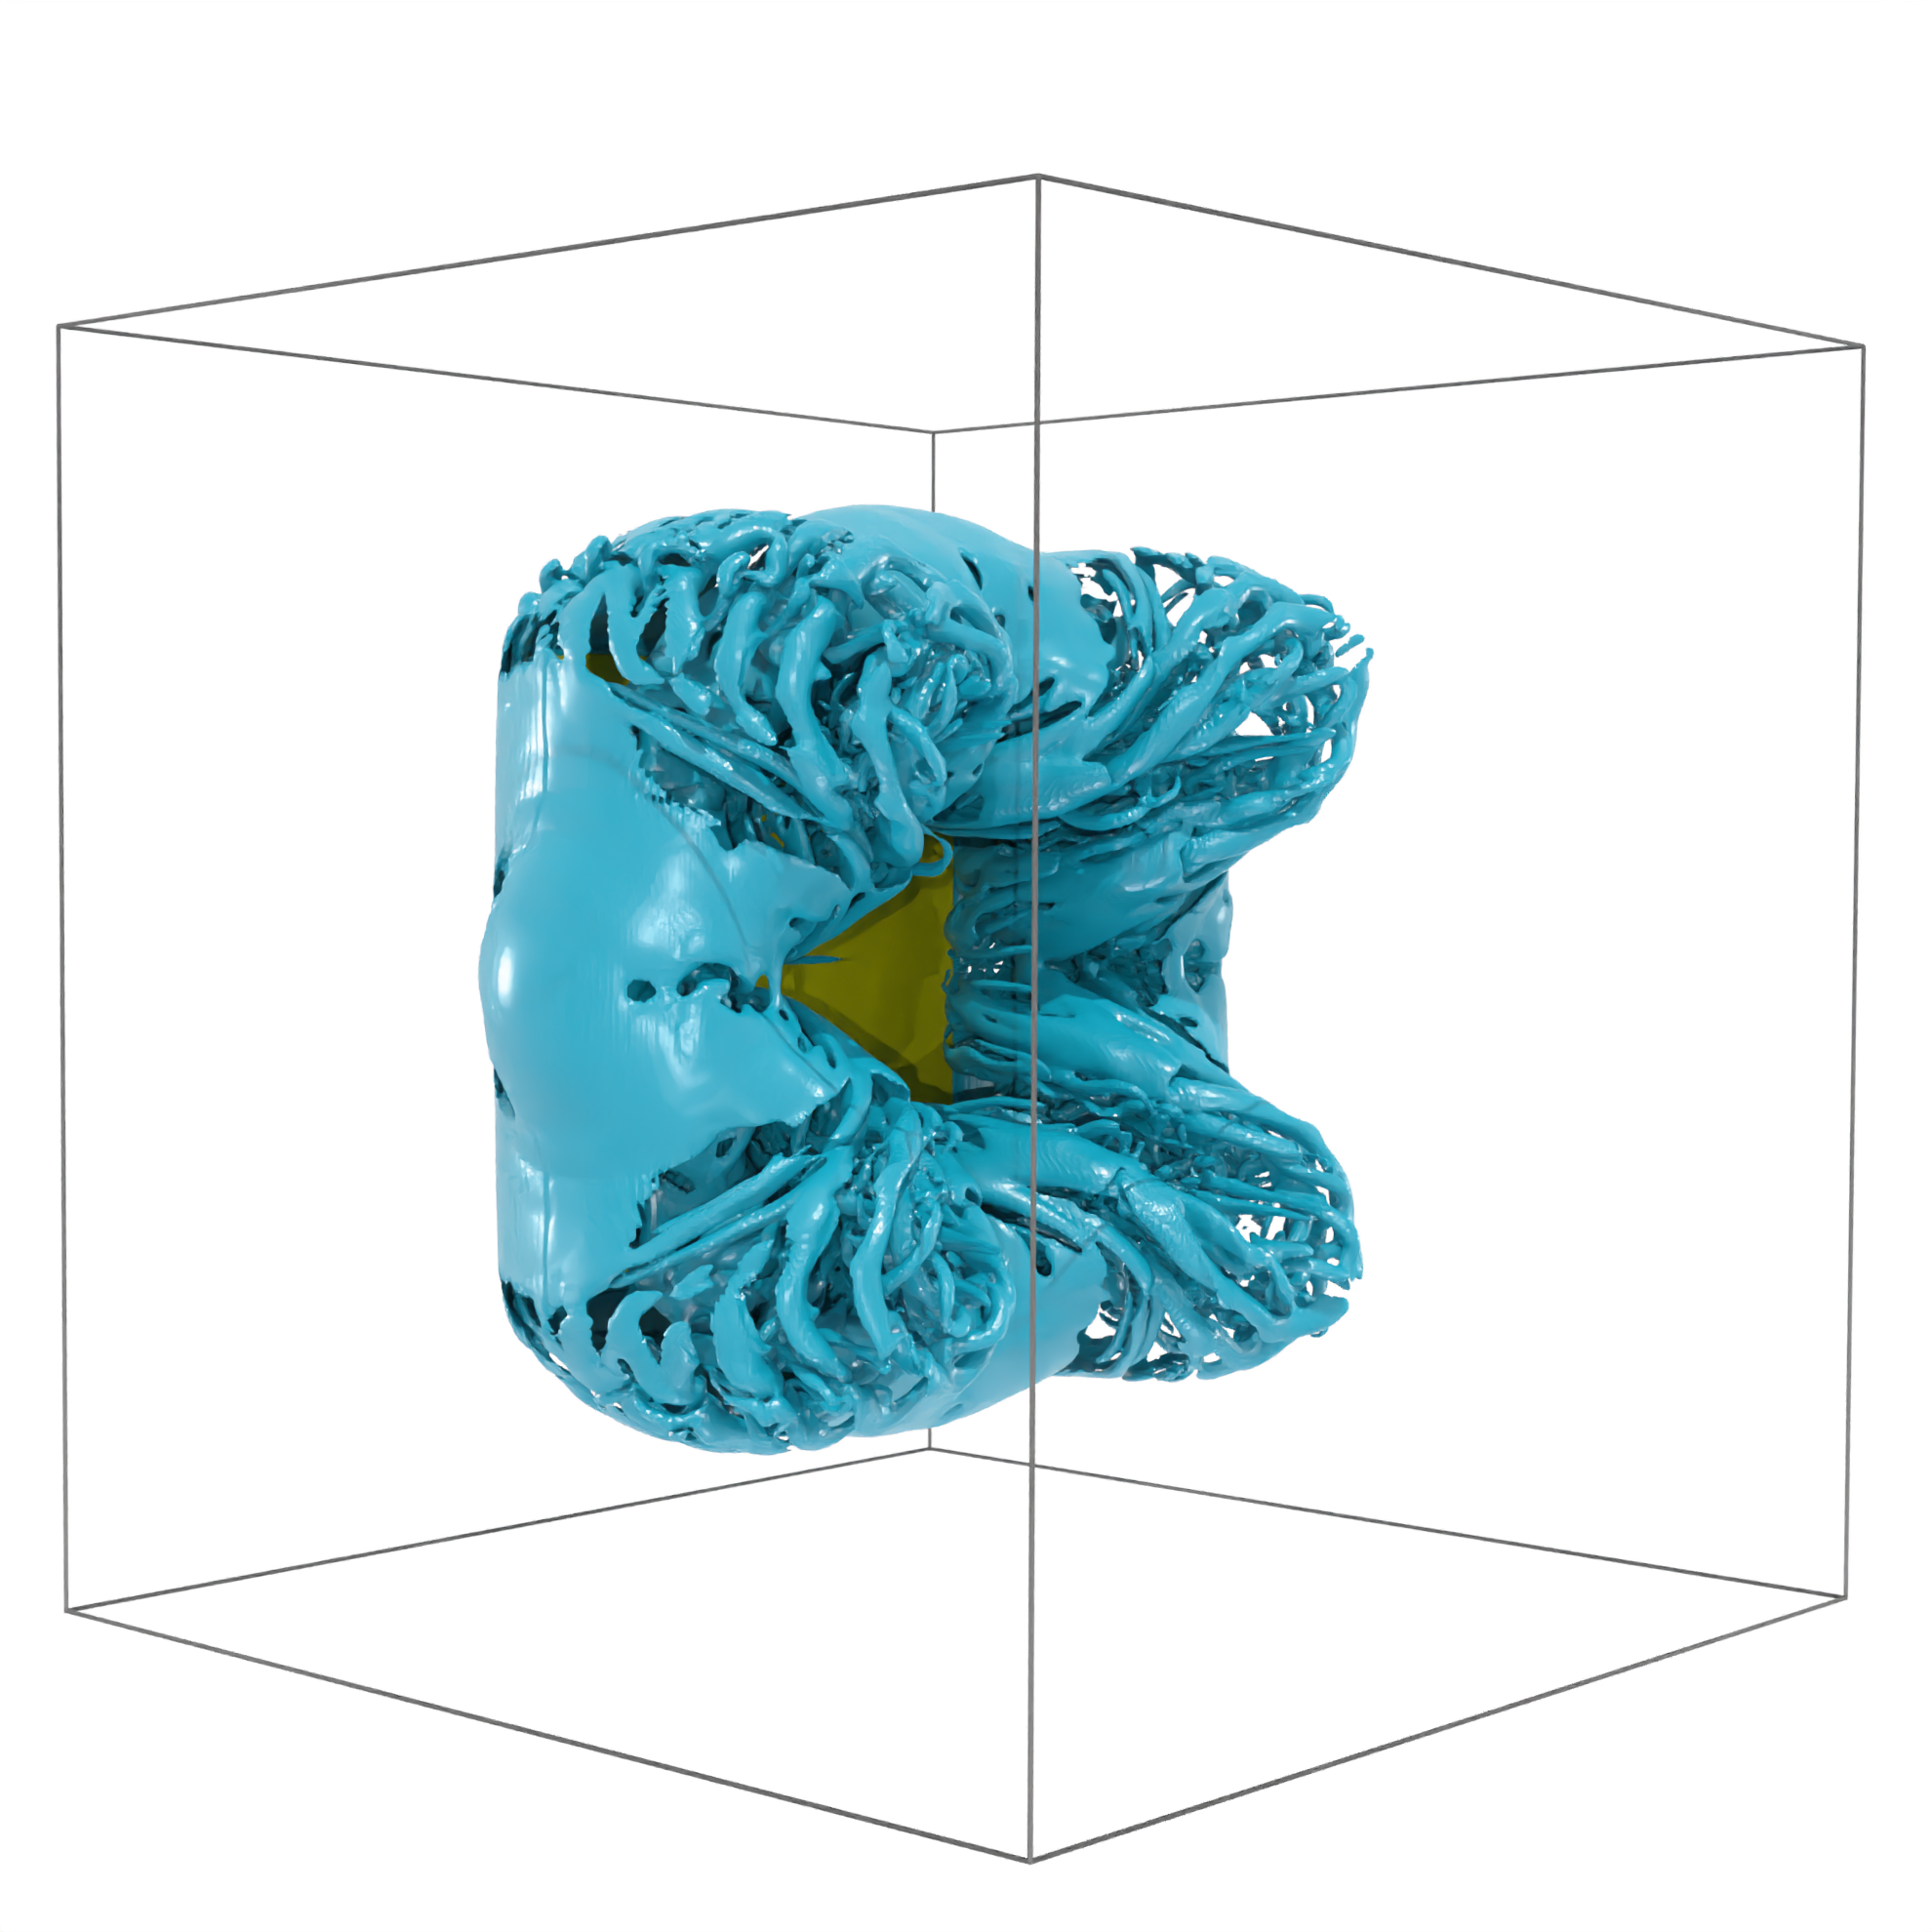
\includegraphics[width=1.1\textwidth]{tex/fig/disk_high_re_7.png}
\end{graphicalabstract}

%%Research highlights
\begin{highlights}
\item External flow boundary condition via the Biot-Savart integral enables minimal computational domains
\item Fast ($\log N$) multilevel evaluation of the Biot-Savart integral with controllable bounded error.
\item Reduction in degrees of freedom by $O(10^3)$ compared to reflection conditions for flow with bounded vorticity. 
\end{highlights}

\begin{keyword}
%% keywords here, in the form: keyword \sep keyword
Biot-Savart \sep Boundary Condition \sep Projection Method \sep Unbounded Domains
%% PACS codes here, in the form: \PACS code \sep code
\PACS 0000 \sep 1111
%% MSC codes here, in the form: \MSC code \sep code
%% or \MSC[2008] code \sep code (2000 is the default)
\MSC 0000 \sep 1111
\end{keyword}

\end{frontmatter}

%% \linenumbers

%% main text

\section{Introduction}
% introduce the problem
Computational fluid dynamics provides a numerical solution to a continuum problem in an (often) unbounded domain. Common practice is to approximate the continuum problem with a discrete set of equations and truncate the unbounded domain to a finite computational domain. 
While the former does not usually introduce significant errors, the latter can significantly impact the numerical solution when the finite domain is not \emph{sufficiently large}. In the context of external flows, \emph{sufficiently large} means that the decaying potential flow induced by the body and the advection/diffusion of vorticity through the domain's boundary have no influence the forces experienced by the body \cite{Colonius2008}.

% introduce why we need far-field BCs
Numerical simulations of external incompressible flows enforce \emph{far-field} boundary conditions on the computational domain's exterior. These consist of a known velocity normal to the boundary and a known normal pressure gradient\footnote{for a description of the boundary conditions for the incompressible \emph{Navier-Stokes} equations, we refer the reader to \cite{Gresho1987}}. These can lead to significant errors. In particular, the force acting on a body can suffer from severe \emph{blockage effects} when the computational domain is not sufficiently large. While domain sensitivity study can determine the extent of the blockage, there is no \emph{a priori} rule for estimating their magnitude, making this an expansive iterative process.

% what have people been doing
Grid stretching away from the immersed body can efficiently maximize the domain size while maintaining a high-resolution mesh around the body, see \cite{Maertens2015, Lauber2022}. This can limit the blockage effects on the body. However, this method requires correct stretching ratios to avoid excessive numerical dissipation or reflection inside the domain. The method is also inefficient in cases where the body undergoes substantial motion within the computational domain, for example, when tracking the motion of a kite. Grid stretching can be replaced by a buffer layer that acts as a numerical damper which ensures that the solution decays rapidly before it reaches the boundaries \cite{Colonius2002ADomains}. Following a similar approach, a coarse grid can provide the boundary conditions for a relatively small, well-resolved domain; this is the basis of the multi-domain methods \cite{Colonius2008}. The method interpolates the coarse mesh solution to the walls of the finer domain, providing artificial far-field boundary conditions.

For flows with one \cite{Grosch1977NumericalTransforms, Levy2022SolvingMethod} or two unbounded directions \cite{Rennich1997NumericalDirections}, coordinate transforms or analytical potential flow solution can be applied in the unbounded directions and correctly capture solution. Potential flow boundary conditions are prescribed following the classical \emph{Helmholtz} decomposition of the velocity field into an irrotational and an incompressible part
\begin{equation}\label{eq:u_vort}
    \vec{u} = \vec{u}_\omega + \nabla\phi + \vec{U}_\infty = -\nabla^{-2}\left(\nabla \times \vec{\omega}\right) + \nabla\phi + \vec{U}_\infty
\end{equation}
where $\vec{u}_\omega$, $\nabla\phi$, $\vec{U}_\infty$ are the incompressible component, irrotational component, and the free-stream velocity, respectively. 
% \begin{equation}\label{eq:u_vort}
%     \vec{u} = \vec{u}_\omega + \nabla\phi + \vec{U}_\infty = -\nabla^{-2}\left(\nabla \times \vec{\omega}\right) + \nabla\phi + \vec{U}_\infty
% \end{equation}
% where $\vec{u}_\omega$ is the vortical component, $\nabla\phi$ is the potential component and $\vec{U}_\infty$ is the free-stream velocity. 

% Fourier-based methods can then be used to solve for the vortical and potential s of the velocity field. Matching the internal and external solution and their derivatives on the domain's boundary closes the system, and the unbounded boundary condition is satisfied on the domain's exterior, at the cost of an augmented system of equations.

% The vortical component is computed by the Fourier solution to the Laplace equation, augmented to capture the zero-mode solution (mean vorticity)
% \begin{equation}\label{eq:u_vort}
%     \vec{u}_\omega = -\nabla^{-2}\left(\nabla \times \vec{\omega}\right).
% \end{equation}
% By solving the Laplace equation $\nabla^2\phi=0$ is cylindrical coordinates via Fourier expansions, the velocity potential can be expressed in terms of Bessel functions of the first and second kind. Matching the internal and external solution and their derivatives on the domain's boundary closes the system, and the unbounded boundary condition is satisfied on the domain's exterior at the cost of an augmented system of equation.

Fundamental solution to discrete operators (Lattice Green's functions or LGFs) and their asymptotic expansions can be used to approximate discrete differential equations on unbounded domains \cite{Liska2014AEquations}. Points close to the source are evaluated with the discrete kernel (accurate) while points far away are evaluated with the asymptotic expansion (fast). These methods rely on the unbounded properties of the LGFs and can simulate unbounded viscous incompressible flow \cite{Liska2016ADomains} and flows with immersed-boundaries \cite{Liska2017AFunctions}. However, they are based on the solution of inhomogeneous, linear, constant coefficient elliptic equations and are thus incompatible with some immersed-boundary methods \cite{Maertens2015, Lauber2022}.

Other methods leverage the strength of an Eulerian-based solver for the near body and Lagrangian solvers for the far wake by coupling a near wall Eulerian solver to a Vortex particle method in the wake \cite{Billuart2023AFlows}. They enable tracking the coarser wake for an extended time while enabling accurate modeling of the developing boundary layer on the object's surface. However, several (user-defined) parameters are required to correctly interpolate the Vortex particle method solution onto the Eulerian mesh. Extension to three-dimensional flow is possible but will significantly increase the computational cost.

All these methods allow for a reduction of the error introduced by truncating an infinite computational domain. However, their generality is often limited to specific discretization of the governing equations or introduces complex coupling procedures.
 
In this manuscript, we propose a novel method for imposing external potential-flow boundary conditions on the velocity and pressure fields on the exterior of a Cartesian computational domain. The method retains the primitive variables formulation ($\vec u$ and $p$) of the covering equations and is compatible with immersed boundaries. Additionally, it does not introduce additional Lagrangian or Eulerian mesh. In the next section, we describe the Biot-Savart boundary conditions and how they are injected into a projection algorithm to solve the \emph{Navier-Stokes} equations. Next, we demonstrate the accuracy of the velocity reconstruction and the balance between speedup and accuracy in the reconstructed field. We then demonstrate, with confined vorticity and vortex-street examples, that the new boundary conditions significantly outperform standard reflective boundary both in terms of computational time and solution accuracy. We present unexpected result that the new method continues to perform well when the fundamental assumption of potential flow external to the domain is violated, and use the unstable deflected wakes generated by fast flapping foils to study the limits of the approach. We close this manuscript with a discussion of the method's applicability to various flows in science and engineering.

\section{Method}

\begin{figure}
    \centering
    \def\svgwidth{0.8\columnwidth}
    \input{fig/domain.pdf_tex}
    \caption{Schematic of the fluid domain $\Omega$ with an immersed body $\mathcal{B}$ and their common (wet) interface $\partial\mathcal{B}$. The exterior of the computational domain $\Omega$ is denoted as $\partial\Omega$ with $\hat{n}$ the unit normal vector.}
    \label{Fig_1}
\end{figure}

We start by describing the governing equations and their numerical solution.
The flow is governed by the \emph{Navier-Stokes} equations for an incompressible flow. We discretize these equations on a staggered finite-volume mesh. The resulting system of equations is solved within a computational domain $\Omega(N)$, where $N$ is the number of degrees of freedom of the problem. The outer domain boundary is denoted at $\partial\Omega(N^{\cal S})$, where $\cal S$ is a factor linked to the dimensions of the problem. In 2D we have $S=1/2$, and in 3D $S=2/3$. The primary source of vorticity in the domain is an immersed body $\mathcal{B}$ with outer (wet) surface $\partial\mathcal{B}$ and unit normal vector $\hat n$, see Figure~\ref{Fig_1}.

We use the standard projection scheme \cite{Chorin1967} to solve the coupled velocity-pressure system inside a predictor-correct method to achieve second-order temporal convergence of the flow variables \cite{Lauber2022}. 
To simplify the discussion, we present the method for the first step of the predictor-corrector; generalization to the second-order Heun's corrector method or higher-order time integration method is straightforward. The projection method starts with an explicit estimate of the intermediate velocity field $u^*$
\begin{align}\label{eq:intermediate}
    \vec{u}^* = \vec{u}\,^t + \int_{t}^{t+\Delta t}\frac{1}{Re}\nabla^2\vec{u} -\left(\vec{u}\cdot\nabla\right)\vec{u}\text{ d}t &\quad\forall\ \vec{x}\in\Omega (N),
\end{align}
where $Re$ is the Reynolds number of the flow. Depending on the choice of integration method for the right-hand-side, we obtain explicit or semi-implicit methods. Here we will focus on fully explicit methods. On the immersed body $
\cal B$, the intermediate velocity is subject to the condition
\begin{equation}
    \vec{u}^* = \vec{U}_b \quad \forall x \in \partial\cal{B}.
\end{equation} 
where $\vec{U}_b$ is the body velocity. Body-fitted methods enforce this condition directly, while immersed boundary methods enforce it indirectly; either by reformulating the governing equations near the boundary such as \cite{Peskin2010,Maertens2015} or by modifying the discretization near $\cal{B}$ \cite{Lee2015}.

Additionally, Eq.~\eqref{eq:intermediate} must be supplemented with far-field boundary conditions on the domain's outer boundaries. As discussed in the introduction, the simplest of these is a reflection condition
\begin{align}\label{eq:BC_1}
    \frac{\partial \vec{u}^*_s}{\partial \hat{n}} = 0,\ \vec{u}^*_n = U_n &\quad\forall\ \vec{x}\in\partial\Omega (N^{\cal S}),
\end{align}
where we have decomposed the velocity field on the boundary in a boundary normal $\vec{u}^*_n$ and tangential part $\vec{u}^*_s$. We refer the reader to \cite{Gresho1987} for a discussion of pressure boundary conditions on the domain's exterior.

Projection of the divergent velocity field onto the solenoidal space is achieved by computing a pressure field $p$ that removes the divergent part of the intermediate velocity field
\begin{align}\label{eq:poisson}
      &\nabla\cdot\frac{\Delta t}{\rho}\nabla p = \nabla\cdot \vec{u}^* &\quad\forall\ \vec{x}\in\Omega (N),\\
      &\vec{u}^{t+\Delta t} = \vec{u}^*-\frac{\Delta t}{\rho}\nabla p &\quad\forall\ \vec{x}\in\Omega (N),
\end{align}
also subject to the standard boundary condition
\begin{align}\label{eq:BC_2}
      &\frac{\partial \vec{u}^{t+\Delta t}_s}{\partial \hat{n}} = 0,\ \vec{u}^{t+\Delta t}_n = U_n &\quad\forall\ \vec{x}\in\partial\Omega (N^{\cal S}).
\end{align}
%Is there a $\partial\Omega$ equation to reduce blockage with $O(N)$ cost?
% We note that Eq.~\ref{eq:poisson} is a variable-coefficient Poisson equation for the pressure (through $\mu_0$), which will become important later in the discussion.
As mentioned previously, the boundary $\partial\Omega$ must be placed sufficiently far away from the body not to influence the fast decaying (potential flow) part of the velocity field and ensure enough space to properly advect the vorticity downstream. 

\subsection{Biot-Savart boundary conditions}

% \begin{figure}
%     \centering
%     \begin{subfigure}{.5\textwidth}
%         \centering
%         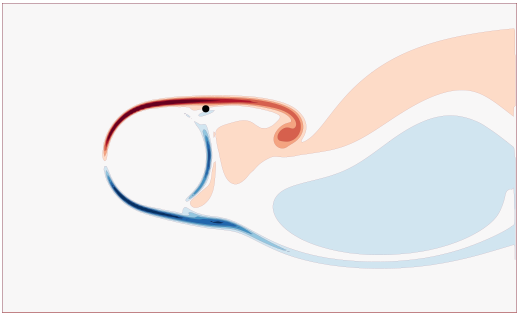
\includegraphics[width=\textwidth]{tex//fig/full_vort.png}
%     \end{subfigure}%
%     \begin{subfigure}{.5\textwidth}
%         \centering
%         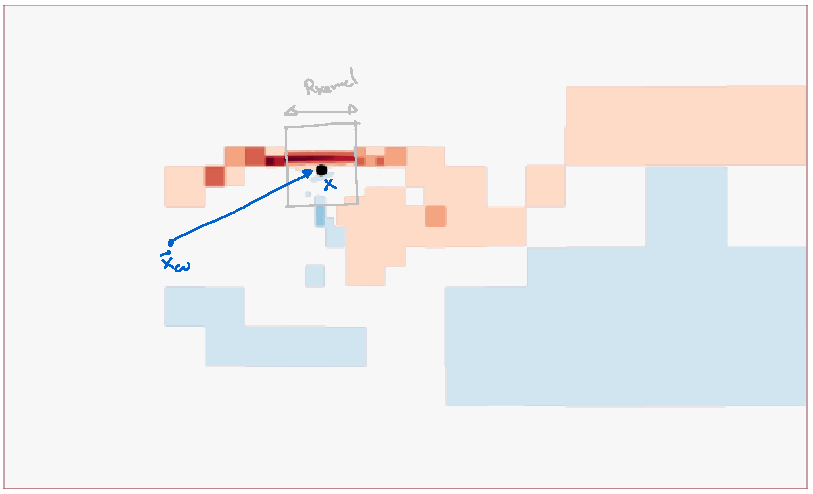
\includegraphics[width=\textwidth]{tex/fig/multilevel_vort.pdf}
%     \end{subfigure}
%     \caption{Vorticity field generated by the flow around a cylinder (left) and the Multilevel approach used to sample the vorticity field for a fast evaluation of the Biot-Savart kernel at the black dot (right).}
%     \label{fig:ml_array}
% \end{figure}

We propose to replace the typical ``local" domain boundary conditions such as Eq.~\eqref{eq:BC_1} \& ~\eqref{eq:BC_2} by a Biot-Savart integral over the vorticity inside the domain. A Green's function solution to the vorticity equation Eq.~\eqref{eq:u_vort} gives the velocity at a point $\vec x$ as
\begin{equation}\label{eq:Biot}
    {\vec u}({\vec x}) = f(\vec x; \vec\omega,\Omega) = \int_\Omega K_{n}({\vec x} - \vec{y})\times \vec\omega({\vec y})\text{ d}\vec{y} \quad\quad \forall \vec x\, \in \partial\Omega (N^{\cal S})
\end{equation}
where $K_n$ is the $n$-dimensional Biot-Savart kernel. This kernel takes the following form \cite{Eldredge2019MathematicalFlows}
\begin{equation}
    2D:\quad K(\vec r)\equiv -\frac{\vec{r}}{2\pi|\vec{r}|^2}, \qquad\qquad 3D:\quad K(\vec r)\equiv -\frac{\vec{r}}{4\pi|\vec{r}|^3}.
\end{equation}

This formulation implicitly assumes the flow external to the domain is irrotational and that the flow is incompressible everywhere. Such a formulation is exact for the flow around accelerated bodies when the time $\frac{tU}{L}\lesssim t^{\text{crit.}}$, with $t^{\text{crit.}}$ the critical time for vortex detachment \cite{Shusser2000EnergyRing}. However, we will show that the results of using equation \eqref{eq:Biot} in an Eulerian solver are still highly accurate for flows with wakes that extend to the domain boundary. 

Note that on a staggered grid, we only need to apply the integral equation \eqref{eq:Biot} to compute the velocity normal to the domain face. For ghost cells external to the computational domain, we use the local derivative conditions $\nabla\cdot\vec{u} = \nabla\times\vec{u}=0$ to compute the velocity. These conditions are consistent with the assumption that the flow is potential outside the domain and fast to apply. Specifically, we apply the zero curl condition to all tangential velocity components in the ghost cells and then the zero divergence condition to the normal components in the ghost cells, marching away from the domain boundary.

% \begin{figure}
%     \centering
%     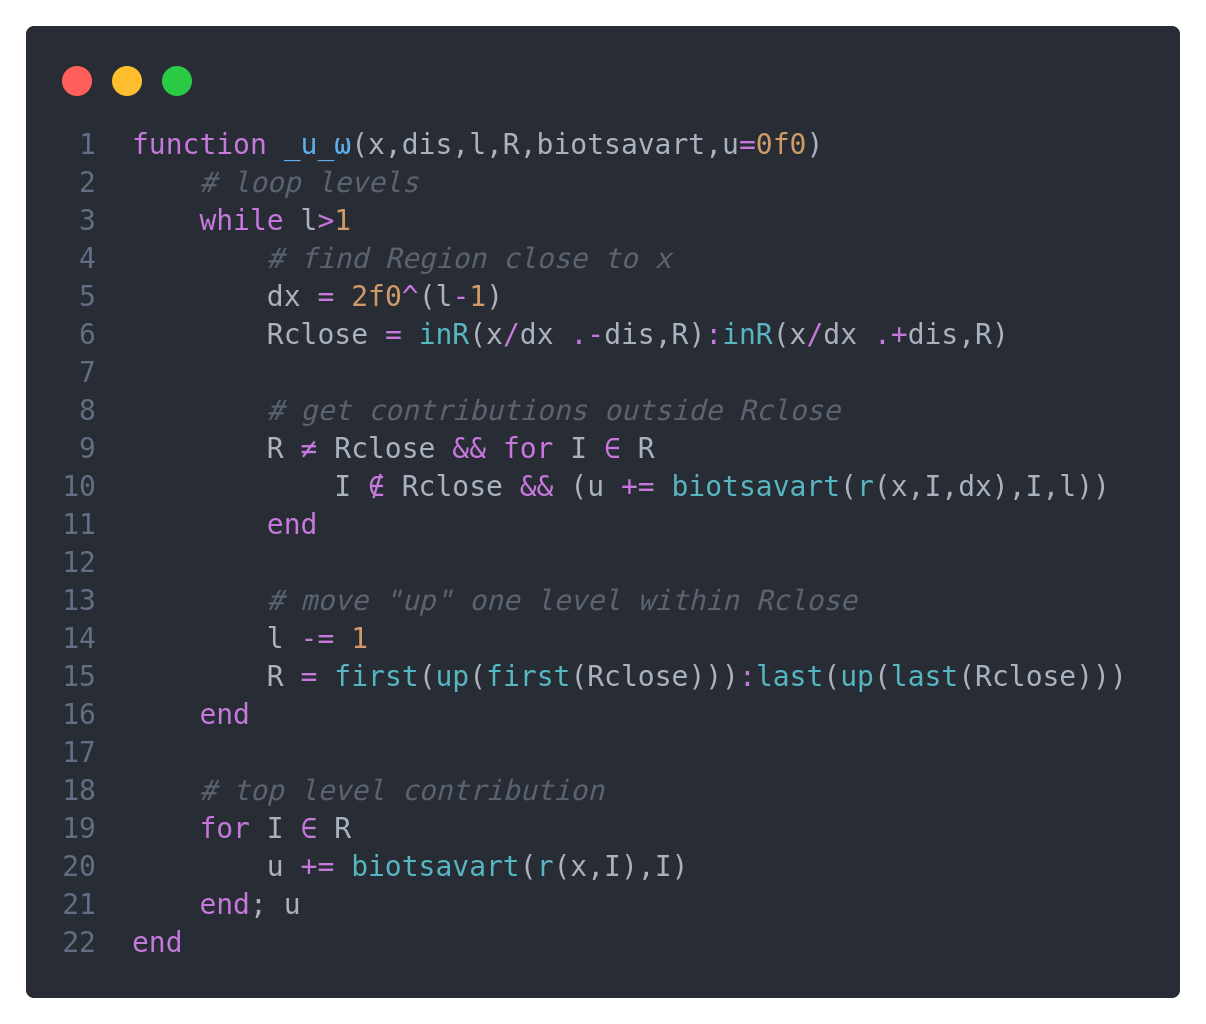
\includegraphics[width=0.5\linewidth]{tex//fig/code.png}
%     \label{fig:code_snippet}
%     \caption{Sample code}
% \end{figure}

\subsection{Fast evaluation of the Biot-Savart integral}

\begin{figure}
    \centering
    \def\svgwidth{0.9\columnwidth}
    \input{fig/multilevel_domain.pdf_tex}
    \caption{Schematic of the multilevel approach to evaluate the Biot-Savart integral for a boundary point $\vec x$ over the nested domains $\mathcal{D}^{(1)} \cup \mathcal{D}^{(2)} \cup \mathcal{D}^{(3)} \cup \mathcal{D}^{(4)}$. The second domain half-width is shown, ${S}^{(2)}$. The computational domain $\Omega$ and its boundary $\partial\Omega$ and the immersed body $\mathcal{B}$ are shown. We also show a schematic of the coarsening of the grid between the domains. Domain and cell size are only for representation proposes.}
    \label{Fig_2}
\end{figure}

The aim of this novel boundary conditions is to reduce the computational cost compared to a large grid by providing an accrate estimate of the far field conditions. A naive evaluation of Eq.~\theequation~ would require $O(N)$ operations \textit{for each boundary point}, meaning $O(N^{1+\cal S})$ cost overall, overwhelming any savings from reducing the size of the domain. In vortex-particle methods, the integral is usually evaluated with \emph{Fast Multipole Method} that allows reducing this cost to $O(\log N)$ operations. Here, we use a multilevel algorithm to achieve the same speed-up in our Eulerian setting.

% This is controlled by a criterion that triggers the evaluation of the velocity on progressively finer meshes. Given a point $x$ where the velocity induced by the vorticity blob located at $x_\omega$, the induced velocity is evaluated on the multilevel if the point $x_\omega$ falls in a box of size $\pm R_\text{kernel}$ around that point, see Fig.~\ref{fig:code_snippet}

We construct the multilevel Biot-Savart operator for each point $\vec x$ on the domain boundary $\partial \Omega$ by representing the complete domain $\Omega$ with a combination of gradually coarser meshes
\begin{equation}\label{eq:multilevel}
    \Omega = \mathcal{D}^{(1)}(\vec x) \cup \mathcal{D}^{(2)}(\vec x) \cup \cdots \cup \mathcal{D}^{(l-1)}(\vec x) \cup \mathcal{D}^{(l)}(\vec x),
\end{equation}
where level $1$ is the finest domain and $l$ is the coarsest, and each domain is non-overlapping and their union fully covers $\Omega$, Fig \ref{Fig_2}. In this work, we define nested rectangular boxes of half-width $S^{(i)}$ centered on $\vec x$ and scale this width with the cell size which doubles at each level, i.e. $
h^{(i)} = h^{(1)} 2^{i-1}$. Therefore the domains are determined by $\vec x$ and a non-dimensional half-width 
\begin{equation}\label{eq:bbox}
    \tilde{S} = \frac{{S}^{(l)}}{2^{l-1}},
\end{equation}
which is equal on every level. This domain decomposition is chosen so that the contributions to Eq.~\eqref{eq:Biot} are more accurately calculated when close to $\vec x$, and the smaller contributions further from $\vec x$ are quickly estimated on the coarser levels.

% Following Eq.~\eqref{eq:multilevel}, the vorticity field in the domain can be expressed as a combination of gradually coarser vorticity fields
% \begin{equation}
%     \omega = \omega^{(1)} \cup \omega^{(2)} \cup \cdots \cup \omega^{(l-1)} \cup \omega^{(l)}
% \end{equation}
% In constructing these fields, it is desirable that some moments of vorticity are conserved to machine precision \cite{Colonius2008}. Our multilevel implementation conserves the total circulation in the domain by a uniform pooling operator
% \begin{equation}
%     \vec{\omega}^{(i)} = \mathcal{P}^{(i-1)\to(i)}\vec{\omega}^{(i-1)} \quad \forall\  \vec{y}\ ^{(i)} \in \mathcal{D}^{(i)}
% \end{equation}
% where $\omega^{(1)}$ is the original finest level field and the pooling $\mathcal{P}$ for a cell at level $i$ simply sums over the corresponding subcells in level $i-1$, see \cite{Weymouth2022Data-drivenProjection}.

With this set of $l$ non-overlapping domains $\mathcal{D}^{(i)}$, the integral in Eq.~\ref{eq:Biot} can be replaced with a sum over all the contribution from the domains
\begin{equation}\label{eq:biot_sum}
    f(\vec{x}; \vec{\omega},\Omega) \approx \sum_{i=1}^{l} f(\vec{x}; \vec \omega^{(i)},\mathcal{D}^{(i)}).
\end{equation}
Once the multilevel field $\omega^{(i)}$ is computed, the total number of operations to evaluate equation \ref{eq:biot_sum} for a simulation of dimension $d=2$ or $3$ is therefore $O(l \tilde S^d)=O(\log N)$ since $\tilde S$ is constant and $l=O(\frac 1 d \log N)$. 

% We see above that the computational cost grows with the subdomain size $\tilde S$, but we show next that this parameter also bounds the multilevel error. We aim to derive an expression for the error in the induced velocity at a point $\vec x$ by evaluating the integral on gradually coarser meshes assuming that the vorticity field on the finest level is exact. 
%In our multilevel algorithm, cells sufficiently far away are grouped with their neighbors to form a cell 4 times bigger in 2D and 8 times bigger in 3D. For simplicity, we discuss the 2D case. Extension to the 3D case is trivial and only requires alternating the out-of-plane vector and using the corresponding vorticity component.

In practise, we use the circulation over a cell face $\Gamma=\omega h^2$ instead of the vorticity in the Biot-Savart formulation. The circulation on a coarser level is calculated by uniformly pooling the circulation on the level above 
\begin{equation}
\Gamma^{(i+1)}=\mathcal{P}^{(i)\to(i+1)}\Gamma^{(i)}
\end{equation}
where $\Gamma^{(1)}$ is the original finest level field and the pooling $\mathcal{P}$ for a cell at level $i$ simply sums over the corresponding subcells in level $i-1$, see \cite{Weymouth2022Data-drivenProjection}. Thus, our multi-level field $\Gamma^{(i)}$ conserves the total circulation to machine precision, as recommended by  \cite{Colonius2008} and others.

Finally, we derive the error induced by this multilevel approach, starting with the 2D-case and extending the result to 3D. The velocity at location $\vec x$ induced by the circulation from a single cell on level $i+1$ is given by (see Fig.~\ref{Fig_2})
\begin{equation}\label{eq:induced_1}
    \vec{u}^{(i+1)}(\vec{x}) = \frac{\vec{r}}{2\pi|\vec{r}|^2}\times\vec{e}_z\mathcal{P}^{(i)\to(i+1)}\Gamma^{(i)}
\end{equation}
where $\vec{r}=\vec{y}-\vec{x}$, $y$ is the center of the cell, and $\vec{e}_z$ is the out-of-plane unit vector. The velocity induced by the four corresponding cells on level $i$ is
\begin{equation}
    \vec{u}^{(i)}(\vec{x}) = \mathcal{P}^{(i)\to(i+1)}
    % \sum_{j\in\mathcal{D}^{(i)}}
    \left(\frac{\vec{r}_j}{2\pi|\vec{r}_j|^2}\times\vec{e}_z\Gamma^{(i)}_j\right),
\end{equation}
where $\vec{r}_j=\vec{y}_j-\vec{x}$ and $y_j$ are the four cell centers. We can further decompose this expression by noting that $\vec{r}_j=\vec{y}-\vec{x}-\vec{\delta r}_j=\vec{r}-\vec{\delta r}_j$.
%, where $\vec{y}$ is the position of the geometric center of the 4 point vortices. 
% Substitution in Eq.~\theequation~ gives
% \begin{equation}
    % \vec{u}^{(i)}(\vec{x}) = \sum_{i\in\mathcal{D}^{(i)}}\frac{\vec{r}-\vec{\delta r}_i}{2\pi|\vec{r}-\vec{\delta r}_i|^2}\times\vec{e}_z\Gamma^{(i)}_i.
% \end{equation}
For sufficiently large $\vec{r}$ we can assume that $|\vec{r}|\approx|\vec{r}-\vec{\delta r}_j|$ %and thus we have
% \begin{equation}
%     \vec{u}^{(i)}(\vec{x}) = \sum_{i\in\mathcal{D}^{(i)}}\frac{\vec{r}-\vec{\delta r}_i}{2\pi|\vec{r}|^2}\times\vec{e}_z\Gamma_i.
% \end{equation}
which allows us to separate the kernel's influence into two parts
% \begin{equation}
%     \vec{u}^{(i)}(\vec{x}) = \sum_{j\in\mathcal{D}^{(i)}}\frac{\vec{r}}{2\pi|\vec{r}|^2}\times\vec{e}_z\Gamma^{(i)}_j-\sum_{j\in\mathcal{D}^{(i)}}\frac{\vec{\delta r}_j}{2\pi|\vec{r}|^2}\times\vec{e}_z\Gamma^{(i)}_j.
% \end{equation}
\begin{equation}
    \vec{u}^{(i)}(\vec{x}) = \mathcal{P}^{(i)\to(i+1)}    \left(\frac{\vec{r}}{2\pi|\vec{r}|^2}\times\vec{e}_z\Gamma^{(i)}_j-\frac{\vec{\delta r}_j}{2\pi|\vec{r}|^2}\times\vec{e}_z\Gamma^{(i)}_j\right).
\end{equation}
After rearrangement, the first term equals Eq.~\eqref{eq:induced_1}. The second term is the error due to the multilevel approximation. Its magnitude is
% \begin{equation}
%     \varepsilon(\vec{x})^{(i)} = \sum_{j\in\mathcal{D}^{(i)}}\frac{\vert\vec{\delta r}_j\vert}{2\pi|\vec{r}|^2}\Gamma^{(i)}_j,
% \end{equation}
\begin{equation}
    \varepsilon(\vec{x})^{(i)} = \mathcal{P}^{(i)\to(i+1)}\frac{\vert\vec{\delta r}_j\vert}{2\pi|\vec{r}|^2}\Gamma^{(i)}_j,
\end{equation}
as $\vec{e}_z$ is a unit vector. On uniform Cartesian meshes, $\vert\vec{\delta r}_j^{(i)}\vert\sim2^{l}$, while $|\vec{r}|^2 \sim (2^l\tilde{S})^2$. An upper bound for the total error in the induced velocity at a point $\vec x$ due to the $i$th-level evaluation of the Biot-Savart integral is therefore
\begin{equation}
    \varepsilon(\vec{x}) \approx \frac{1}{2\pi\tilde{S}^2}\sum_{i=2}^{l}\frac{1}{2^i}\mathcal{P}^{(i)\to(i+1)}
    % \sum_{i\in\mathcal{D}^{(i)}}
    \Gamma^{(i)}.
\end{equation}
which decays as $\tilde{S}^{-2}$. The content of each sum is a decreasing fraction of the total vorticity contained in the domain $\mathcal{D}^{(i)}$. As expected, taking $\tilde{S}>\text{Domain}$ yields $\varepsilon(\vec{x}) = 0$, and as $\Gamma^{(i)} \to 0, \varepsilon(\vec{x})\to 0$, finally as $\tilde{S}\to0, \varepsilon(\vec{x}) \to \infty$. Similarly, in 3D the upper bound for the error is given by
\begin{equation}
    \varepsilon(\vec{x}) \approx \frac{1}{4\pi\tilde{S}^3}\sum_{i=2}^{l}\frac{1}{2^{2i}}\mathcal{P}^{(i)\to(i+1)}
    % \sum_{j\in\mathcal{D}^{(i)}}
    \Gamma^{(i)}.
\end{equation}
which decays as $\tilde{S}^{-3}$. Similarly, the content of the sum is a (even smaller) decreasing fraction of total vorticity contained in each level, improving the method's accuracy in 3D compared to 2D.

% The cost of the evaluation of the Biot-Savart integral is also proportional to the bounding box dimension. Each level contains approximately $\tilde{S}^d$ points, with $d$ the dimension of the problem. Using a $l$-level mutligrid will result in roughly $\tilde{S}^d\times l$ operations. The maximum number of levels is given by $l=N/\tilde{S}$. The total cost is thus $\tilde{S}^{d-1}N$ which is much lower than the total number of operations required to evaluate Eq.~\eqref{eq:Biot} without a multilevel approach.


% Let $\vec{S}^{l}$ be the distance criterion on level $l$, the total error is a sum of all the errors in the $N_l$ lower level of the multilevel
% \begin{equation}
%     \varepsilon^{(1)}(\vec{x}) = \sum_{l=2}^{N_l}\frac{\sqrt{2}\Delta x^{(l-1)}}{4\pi|\vec{S}^{(l-1)}|^2}\sum_{i=1}^{4l}\Gamma_i.
% \end{equation}

% As expected, taking $\vec{S}>\text{Domain}$ yiels $\varepsilon^{(1)}(\vec{x}) = 0$, and as $\Gamma_i \to 0, \varepsilon^{(1)}(\vec{x})\to 0$, finally as $|\vec{S}|\to0, \varepsilon^{(1)}(\vec{x}) \to \infty$. Similarly, in 3D the error is given by
% \begin{equation}
%     \varepsilon^{(1)}(\vec{x}) = \sum_{l=2}^{N_l}\frac{\sqrt{3}\Delta x^{(l-1)}}{16\pi|\vec{S}^{(l-1)}|^3}\sum_{i=1}^{8l}\Gamma_i,
% \end{equation}
% which decays much faster than in 2D.

% The integral in Eq.~\ref{eq:Biot} is then evaluated by the recursive expression, starting from the lowest level of the multilevel
% \begin{equation}
%     f^{(i)}(\vec{x},\vec{y},\vec{\omega}^{(l)}) = \begin{cases}
%         \sum_{\vec{y}\in\mathcal{D}^{(l)}}K^{(l)}(\vec{x},\vec{y},\vec{\omega}^{(l)}), \quad \forall \,\, \vec{y} \in \mathcal{D}^{(l)}\\
%         f^{(l-1)}(\vec{x},\vec{y},\vec{\omega}^{(l-1)}), \,\,\qquad \text{else},
%     \end{cases}
% \end{equation}
% where $K^{(l)}(\vec{x},\vec{y},\vec{\omega}^{(l)})$ is the discrete Biot-Savart kernel at level $l$ and the criterion $\vec{y} \in \mathcal{D}^{(l)}$ is evaluated using a standard cut-of radius.
% \begin{equation}
%     \begin{cases}|\vec{y}-\vec{x}|/2^l<|\vec{S}|, \qquad \vec{y} \in \mathcal{D}^{(l)},\\
%     |\vec{y}-\vec{x}|/2^l>|\vec{S}|, \qquad \vec{y} \notin \mathcal{D}^{(l)}.
%     \end{cases} 
% \end{equation}

% \textbf{Must be a bounding box and not a cut-off radius}
% \textbf{Still need to show the cost to evaluate integral is logN. $S^2*l$}

\subsection{Biot-Savart \& Projection Algorithm}\label{sec:Biot_projection}
Substitution of the Biot-Savart boundary condition (Eq.~\ref{eq:Biot}) into the projection scheme results in a slightly modified intermediate velocity field\\
\textbf{Biot-Savart intermediate step}
\begin{align}
    &\vec{u}^* = \vec{u}\,^t + \int_{t}^{t+\Delta t}\frac{1}{Re}\nabla^2\vec{u} -\left(\vec{u}\cdot\nabla\right)\vec{u}\text{ d}t &\quad\forall\ \vec{x}\in\Omega (N),\\
    &\vec{u}^* = f(\vec{x}_b,\nabla\times \vec{u}^*,\Omega) &\quad\forall\ \vec{x}_b\in\partial\Omega (N^{\cal S})
\end{align}
where the exterior boundary condition have been computed from the intermediate velocity $\vec{u}^*$ in the domain. The projection step, however, results in a coupling between the body and the domain's boundary through the pressure field
\begin{align}
  &\nabla\cdot\frac{\Delta t}{\rho}\nabla p = \nabla\cdot \vec{u}^* \\
  %\forall\ \vec{x}\in\Omega (N)\\
  &\vec{u}^{t+\Delta t} = \vec{u}^*-\frac{\Delta t}{\rho}\nabla p \\
  %\quad\forall\ \vec{x}\in\Omega (N)\\
  &\vec{u}^{t+\Delta t} = f(\vec{x},\nabla\times \vec{u}^{t+\Delta t},\Omega)= \vec{u}^*-f(\vec{x}_b,\nabla\times\frac{\Delta t}{\rho}\nabla p,\Omega) 
  %\quad\forall\ \vec{x}\in\partial\Omega (N^{\cal S}).
\end{align}
Where we have omitted the domain of definition of each equation for clarity. Away from the body, the source term in the Biot-Savart integral in Eq.~\theequation~ vanishes. However, due to the pressure boundary condition on the immersed body ($\partial p/\partial\hat{n}=\hat{n}\cdot(\nabla^2\vec{u}/Re-\text{D}\vec{U}_b/\text{D}t)$), a thin layer of vorticity is generated by the pressure gradient term that changes the induced velocity field on the outer domain's boundary. The projection steps and the Biot-Savart boundary conditions now form a fixed-point system

\textbf{Biot-Savart projection step}
\begin{align}
    &\nabla\cdot\frac{\Delta t}{\rho}\nabla p = \nabla\cdot \vec{u}^*-\nabla\cdot f(\vec{x}_b,\nabla\times\frac{\Delta t}{\rho}\nabla p,\Omega)\\
    %\quad\forall\ \vec{x}\in\Omega, \vec{x}_b\in\partial\Omega\ (N^{\cal S})\\
    &\vec{u}^{t+\Delta t} = \vec{u}^*-\frac{\Delta t}{\rho}\nabla p\\ 
    %\qquad\qquad\qquad\qquad\qquad\forall\ \vec{x}\in\Omega (N)\\
    &\vec{u}^{t+\Delta t} = f(\vec{x},\nabla\times \vec{u}^{t+\Delta t},\Omega)= \vec{u}^*-f(\vec{x}_b,\nabla\times\frac{\Delta t}{\rho}\nabla p,\Omega)
    %\quad\forall\ \vec{x}_b\in\partial\Omega (N^{\cal S}).
\end{align}
This coupling only occurs on the domain's boundary, and the resulting system is mildly non-linear. This weak non-linearity can be solved efficiently with a deferred correction approach, which explicitly updates the source term of the Poisson problem during each pressure solver iteration. This coupling is only apparent in immersed boundary methods if the pressure boundary conditions are correctly imposed on the immersed body during the projection step; see for example \cite{Taira2007, Lauber2022}.

Lastly, we note that the small multilevel error discussed in the previous section means that global mass conservation is no longer guaranteed on the domain boundary. As such, we apply a uniform correction
\begin{equation}
    \vec{u} = \vec{u} -\frac {\oint_{\partial\Omega }\hat{n}\cdot\vec{u}\text{ d}S} {\oint_{\partial\Omega }\text{ d}S}.
\end{equation}
ensuring a globally divergence-free field is passed to the pressure projection method.

\section{Multilevel reconstruction validation}

We start by validating the multilevel reconstruction algorithm presented above. We selected to cases such respect our assumption of vorticity being confined far from the domain's boundary. We demonstrate the 2D and 3D reconstruction error of the multilevel and the speedup generated by selecting the correct kernel radius from the above analysis.

Our Biot-Savart boundary conditions are implemented inside \textbf{\color{cyan}{{WaterLily.jl}}}\footnote{\url{https://github.com/weymouth/WaterLily.jl}}, a fast, immersed-boundary flow solver based on the Boundary data immersion method \cite{Maertens2015} that can execute both on CPU and GPU \cite{Weymouth2023WaterLily.jl:Execution}. To leverage the GPU capability of the flow solver and fully benefit from our novel boundary conditions, we perform all computations presented herein on an NVIDIA-A6000 GPU (48GB memory). All the codes used for this study and the instructions to reproduce these results are freely available at \url{https://github.com/weymouth/BiotSavartBCs.jl}.

\subsection{2D validation: Lamb vortex}

The velocity field generated by the Lamb-Chaplygin dipole is obtained from the scalar stream function $\vec{u} = -\vec{e}_z\times \nabla \psi$ given by
\begin{equation}
    \psi(r) = \begin{cases}
    \frac{-2UJ_1(\beta r)}{\beta J_0(\beta R)}, \quad \text{for} \quad r < R,\\
    U\left(\frac{R^2}{r}-r\right), \quad \text{for} \quad r \ge R,    \end{cases}
\end{equation}
%Meleshko, V. V.; Heijst, G. J. F. van (August 1994). "On Chaplygin's investigations of two-dimensional vortex structures in an inviscid fluid". Journal of Fluid Mechanics. 272: 157–182. Bibcode:1994JFM...272..157M. doi:10.1017/S0022112094004428. ISSN 1469-7645. S2CID 123008925.
where $J_0$ and $J_1$ are the zeroth and first Bessel functions of the first kind, respectively. $\beta$ is a parameter with the value $\beta=1.2197\pi/R$. The core of the vortex is defined by the isoline $\psi(r=R)=0$, that delimits the inside and outside of the vortex.

\begin{figure}
\begin{subfigure}{.5\textwidth}
  \centering
  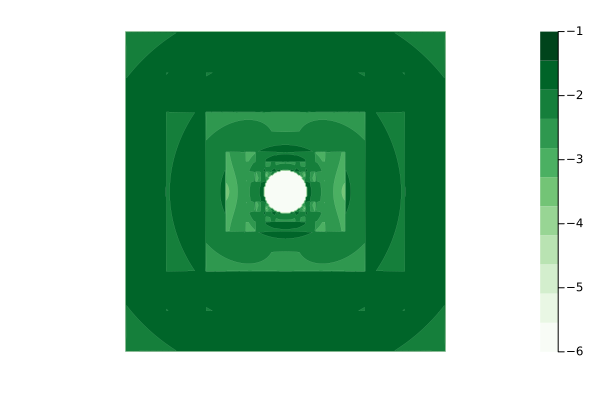
\includegraphics[width=\linewidth]{tex/fig/lamb_dipole_error_dist2.png}
  \caption{$\log(\text{size})=1$}
\end{subfigure}%
\begin{subfigure}{.5\textwidth}
  \centering
  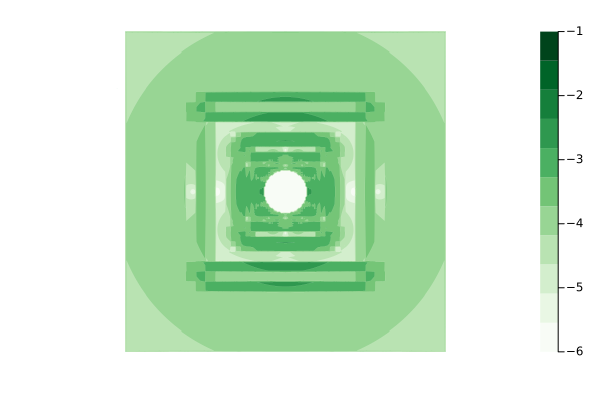
\includegraphics[width=\linewidth]{tex/fig/lamb_dipole_error_dist8.png}
  \caption{$\log(\text{size})=3$}
\end{subfigure}
\begin{subfigure}{.5\textwidth}
  \centering
  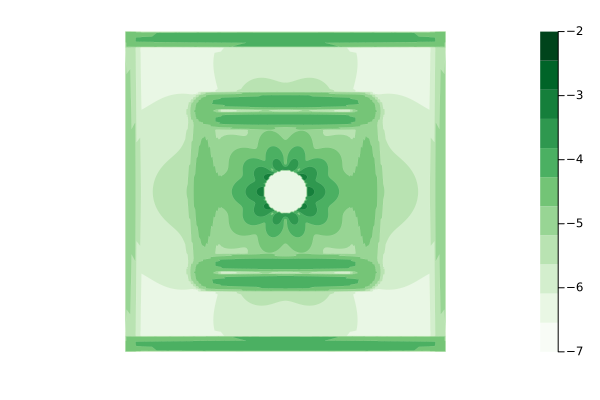
\includegraphics[width=\linewidth]{tex/fig/lamb_dipole_error_dist32.png}
  \caption{$\log(\text{size})=5$}
\end{subfigure}%
\begin{subfigure}{.5\textwidth}
  \centering
  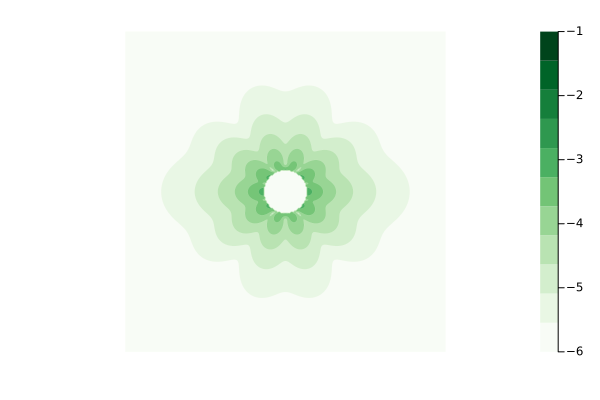
\includegraphics[width=\linewidth]{tex/fig/lamb_dipole_error_dist128.png}
  \caption{$\log(\text{size})=8$}
\end{subfigure}
\caption{$L_2$-norm of the error in reconstructed velocity field outside the core of the 2D Lamb-Chaplygin vortex for varying (multi-level) kernel size. Error bars are shown in log-scale.}
\label{fig:lam_error_dist}
\end{figure}

We reconstruct the velocity field outside the vortex core using the internal vorticity and our multilevel Biot-Savart method and compare that to the analytic result. We reconstruct the velocity on a domain of size $[2^8,2^8]$. The dependency of the absolute error in the reconstructed velocity field on the radius of the multilevel refinement criterion are shown in Fig.~\ref{fig:lam_error_dist}. Setting the refine size $\tilde{S}$ to the domain size $\cal D$ eliminates the multi-level-error, but the result is not exact since the analytic vorticity distribution is sampled on a finite grid of size $\Delta x=0.05
R$. This error depends primarily on the distance from the vortex, Fig.~\ref{fig:lam_error_dist}(d). Progressively reducing the refinement size $\tilde{S}$ introduces the multilevel error quantified in the previous section, which is only weakly dependent on the distance to the vortex.

This is further quantified in Fig.~\ref{fig:error_lamb_2}(a), which shows the maximum error in the reconstructed velocity field at a distance $d$ from the vortex from the Lamb-Chaplygin vortex. The size $\tilde{S}$ is shown to dominate the reconstruction error, with fairly uniform total error levels once $\tilde{S} \le 2^3 = 8$. Fig.~\ref{fig:error_lamb_2}(a) reports the measured computational speed-up achieved by the multilevel method relative to setting $\tilde{S}=\cal D$, demonstrating up to 300$\times$ acceleration.

\begin{figure}
    \centering
    \begin{subfigure}{.5\textwidth}
        \centering
        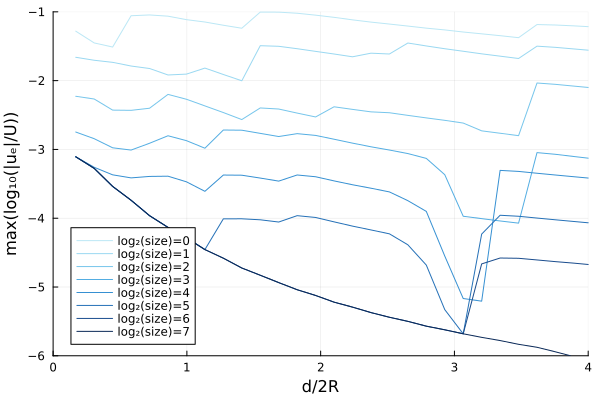
\includegraphics[width=\textwidth]{tex//fig/lamb_dipole_error_dists.png}
    \end{subfigure}%
    \begin{subfigure}{.5\textwidth}
        \centering
        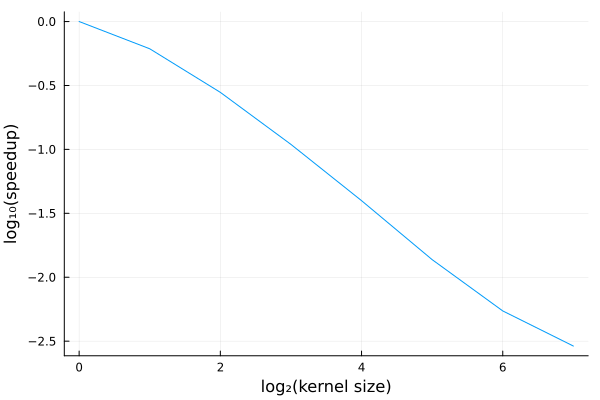
\includegraphics[width=\textwidth]{tex/fig/lamb_dipole_speedup_dists.png}
    \end{subfigure}
    \caption{Maximum error in the reconstructed velocity field generated by a 2D \emph{Lamb-Chaplygin} vortex dipole for various kernel sizes and distances from the vortex core (left). Corresponding speed-up obtained by reducing the kernel size for the multilevel algorithm (right). The mesh has dimensions $[2^8,2^8]$.}
    \label{fig:error_lamb_2}
\end{figure}

\subsection{3D validation: Hill vortex}

This validation is repeated in 3D using the classical \emph{Hill vortex}, whose radial and tangential velocity components are given by
\begin{align}
    v_r &= \frac{1}{r^2\sin\theta}\frac{\partial\psi}{\partial\theta}, \qquad v_\theta = -\frac{1}{r\sin\theta}\frac{\partial\psi}{\partial r}.
\end{align}
and the stream function 
\begin{equation}
    \psi(r,\theta) = \begin{cases}
    -\frac{3U}{4}\left(1-\frac{r^2}{R^2}\right)r^2sin^2\theta \quad \text{for} \, r \le R,\\
     \,\,\frac{U}{2}\left(1-\frac{r^3}{R^3}\right)r^2sin^2\theta \quad \text{for} \, r > R.
    \end{cases}
\end{equation}
with the corresponding errors and speed-up shown in Figure~\ref{fig:error_hill_3}. Note that the analytic vorticity of the hill vortex is discontinuous, increasing the truncation error near the vortex compared to the smooth Lamp-vortex, a problem which would not be observed with any real three-dimensional viscous flow.

As argued in Sec.~\ref{sec:Biot_projection} the multilevel error decreases extremely quickly as $\tilde{S}$ is increased for three-dimensional flows. This is due to the scaling of the Biot-Savart kernel itself. The 3D case demonstrates a stronger sensitivity to the distance to vortex, as expected from the error estimate. Similarly, the speed-up is much faster in 3D because each doubling gathers 8 cells instead of 4, with a max observed speed-up of nearly 20,000$\times$ using the multilevel method.

\begin{figure}
    \centering
    \begin{subfigure}{.5\textwidth}
        \centering
        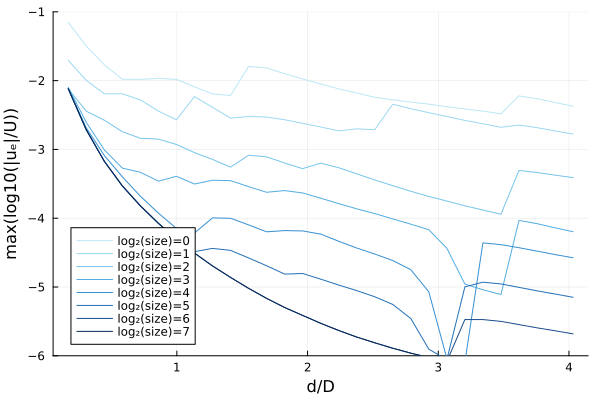
\includegraphics[width=\textwidth]{tex//fig/Hill_error_dists.png}
    \end{subfigure}%
    \begin{subfigure}{.5\textwidth}
        \centering
        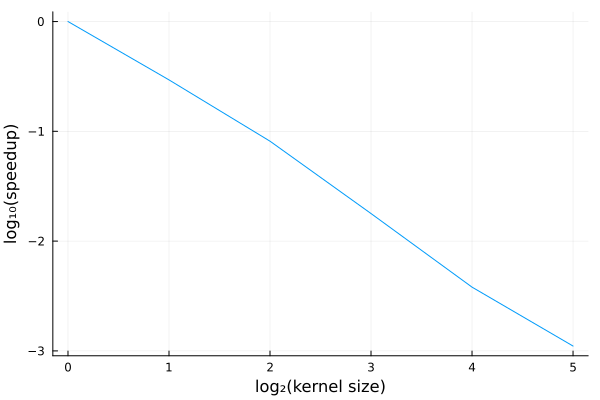
\includegraphics[width=\textwidth]{tex/fig/Hill_speedup_dists.png}
    \end{subfigure}
    \caption{Maximum error in the reconstructed velocity field generated by a 3D \emph{Hill} vortex for various kernel sizes and distances from the vortex core (left). Corresponding speed-up obtained by reducing the kernel size for the multilevel algorithm (right). The mesh has dimensions $[2^8,2^8,2^8]$.}
    \label{fig:error_hill_3}
\end{figure}

\section{Confined vorticity applications}

We next validate the application of the Bio-Savart conditions to the solution of a set of impulsive flow problems. The flow is truly irrotational outside the computational domain, matching the implicit assumptions required to use the Biot-Savart equations to reconstruct the velocity on the boundary. 

\subsection{3D flow around an accelerating disk}

The flow around a disk accelerated from rest in a quiescent flow is purely potential for $t\to 0^+$. As a result, an analytical expression for the added mass coefficient and the pressure field can be used to validate our novel potential flow boundary condition when injected in a moment step of the \emph{Navier-Stokes} equations. We place a disk of radius $R$ in an initially quiescent flow. The disk is prescribed with a constant acceleration $a$ during one non-dimensional time $t^*=at/U$
\begin{equation}
    U(t) = \begin{cases}
        at, \quad \text{if } at/U\le1,\\
        U, \quad \text{else}.
    \end{cases}
\end{equation}
We integrate the Navier-Stokes equation during a single time-step from $t=0\to0^+$ and compute the pressure force acting on the disk for various domain sizes. From potential flow theory, the added-mass coefficient for an impulsively started flow is
\begin{equation}
    Ca  = \frac{F_{am}}{\rho D^3 a} = \frac{F_{am}}{\rho D^2U^2}\left(\frac{1}{a^*}\right) = \frac{1}{3}
\end{equation}
where $Ca$ is the classical added-mass coefficient for a circular plate. We then continue the simulation until $t^*=3$. Once the disk reaches its peak velocity, the Reynolds number is $Re=\frac{UR}{\nu}=1000$.

We note here that the problem possesses two axes of symmetry that would allow only $1/4$ of the domain to be modelled. This can be easily accounted for in the Biot-Savart boundary conditions by adding the contributions of the images of each point. However, with our multilevel approach, they might lie on different levels, rendering the evaluation cumbersome. To avoid unnecessary complications, we model the full plate and do not use the symmetries of the problem.

Figure~\ref{fig:disk_flow_1}-\ref{fig:disk_flow_2} shows the vorticity and pressure field at three consecutive times during the cylinder's motion. Fig.~\ref{fig:disk_flow_1} show the results with the standard reflective boundary conditions (the entire computational domain is shown), and in Fig.~\ref{fig:disk_flow_2}, the flow has been obtained with the Biot-Savart boundary conditions. High blockage effects are apparent for the reflective boundary conditions, with stronger shear layers and a vortex center located further downstream than the Biot-Savart results. The pressure field is even more striking. With iso-contour of the pressure sticking to the wall to satisfy the homogeneous Neumann condition set by the velocity field, see \cite{}. Because the Biot-Savart boundary conditions improve this boundary condition, the pressure follows the expected potential flow solution and, more importantly, is relaxed from the homogeneous Neumann condition that reflective boundary conditions imposed.

\begin{figure}
    \centering
    \begin{subfigure}{.33\textwidth}
        \centering
        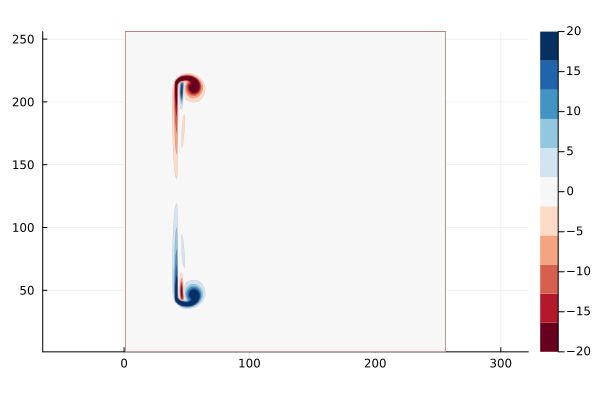
\includegraphics[trim={4cm 7.2cm 5cm 1cm},clip,width=\textwidth]{tex/fig/Disk_reflect_omega_1.png}
        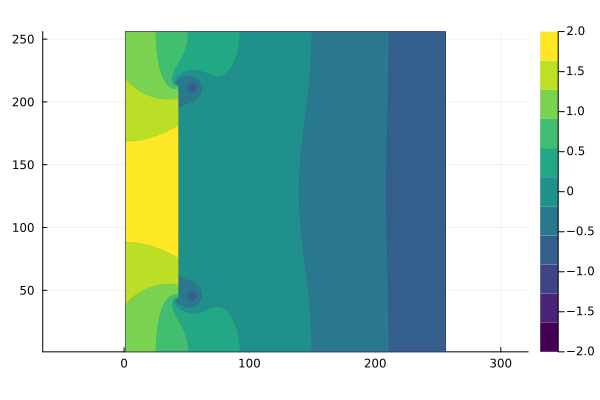
\includegraphics[trim={4cm 1.5cm 5cm 7cm},clip,width=\textwidth]{tex/fig/Disk_reflect_press_1.png}
    \end{subfigure}%
    \begin{subfigure}{.33\textwidth}
        \centering
        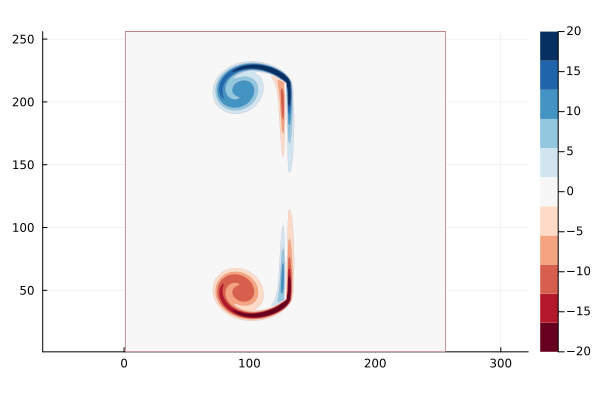
\includegraphics[trim={4cm 7.2cm 5cm 1cm},clip,width=\textwidth]{tex/fig/Disk_reflect_omega_2.png}
        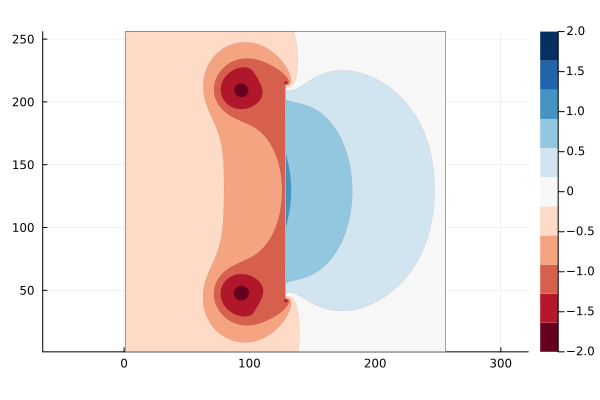
\includegraphics[trim={4cm 1.5cm 5cm 7cm},clip,width=\textwidth]{tex/fig/Disk_reflect_press_2.png}
    \end{subfigure}%
    \begin{subfigure}{.33\textwidth}
        \centering
         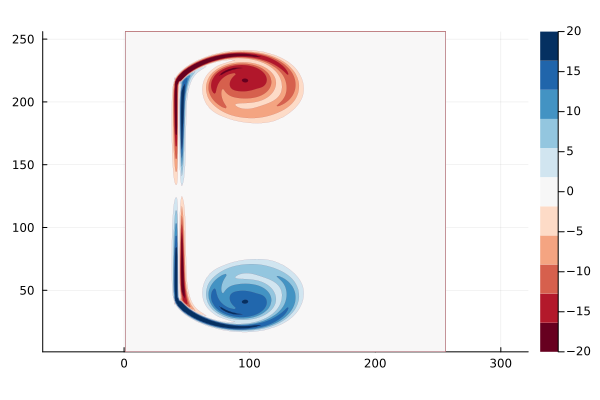
\includegraphics[trim={4cm 7.2cm 5cm 1cm},clip,width=\textwidth]{tex/fig/Disk_reflect_omega_3.png}
        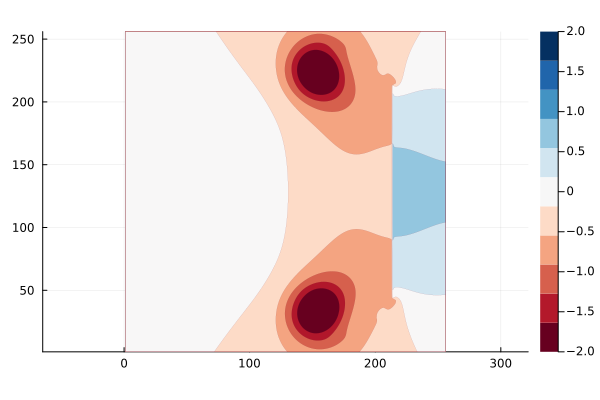
\includegraphics[trim={4cm 1.5cm 5cm 7cm},clip,width=\textwidth]{tex/fig/Disk_reflect_press_3.png}
    \end{subfigure}
    \caption{Flow around an initially stationary disk accelerated in a quiescent flow at three convective times, $t^*\in [1,2,3]$, using the reflective boundary conditions. The entire computational domain is shown. The top half shows 10 iso-contour of the vorticity, equally spaced in the interval $\omega L/U\in\pm20$. The bottom half shows the pressure field, with 10 iso-contour equally spaced in $p/\rho U^2\in\pm2$.}
    \label{fig:disk_flow_1}
\end{figure}

% Zero point for time. Xu and Nietsche paper 2015.

Fig.~\ref{fig:disk_forces} shows the time trace of the pressure force acting on the accelerated disk. The difference in the pressure field is found again in the difference in the forces. Here, the Biot-Savart boundary condition can exactly recover the added-mass force on the first time step, while the reflective boundary condition overestimates it. For larger $t^*$, the effect of the boundary condition is still observable; the reflective boundary condition significantly overestimates the pressure forces

\begin{figure}
    \centering
    \begin{subfigure}{.33\textwidth}
        \centering
         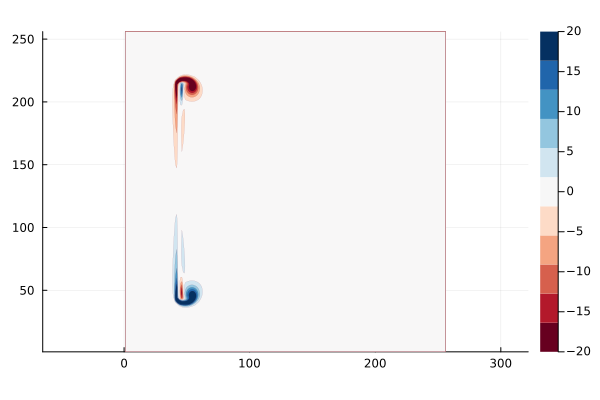
\includegraphics[trim={4cm 7.2cm 5cm 1cm},clip,width=\textwidth]{tex/fig/Disk_biot_omega_1.png}
        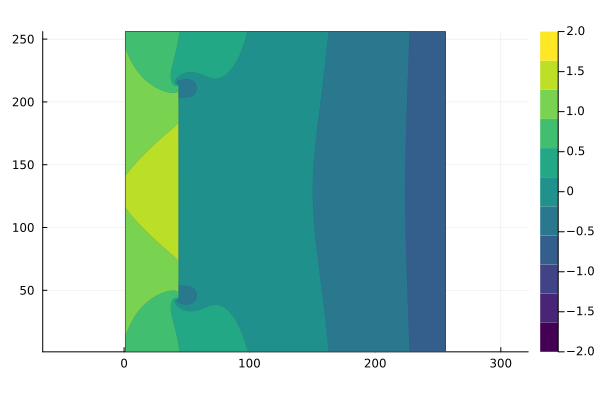
\includegraphics[trim={4cm 1.5cm 5cm 7cm},clip,width=\textwidth]{tex/fig/Disk_biot_press_1.png}
    \end{subfigure}%
    \begin{subfigure}{.33\textwidth}
        \centering
        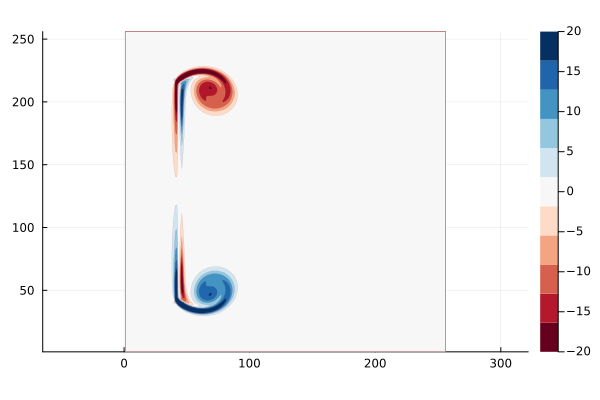
\includegraphics[trim={4cm 7.2cm 5cm 1cm},clip,width=\textwidth]{tex/fig/Disk_biot_omega_2.png}
        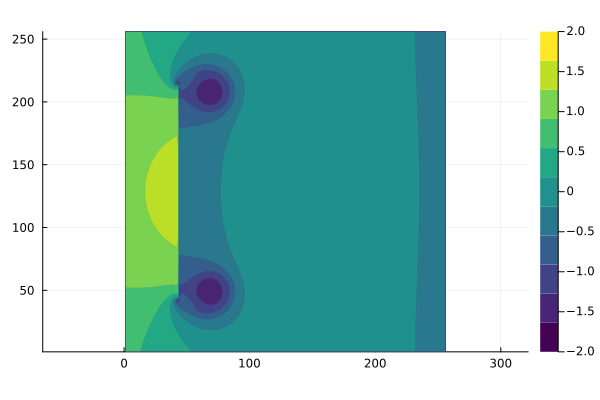
\includegraphics[trim={4cm 1.5cm 5cm 7cm},clip,width=\textwidth]{tex/fig/Disk_biot_press_2.png}
    \end{subfigure}%
    \begin{subfigure}{.33\textwidth}
        \centering
         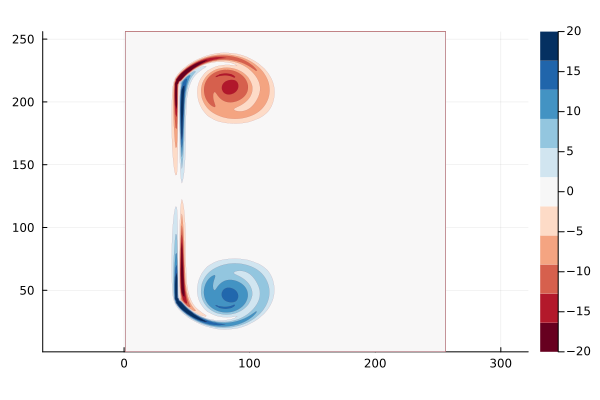
\includegraphics[trim={4cm 7.2cm 5cm 1cm},clip,width=\textwidth]{tex/fig/Disk_biot_omega_3.png}
        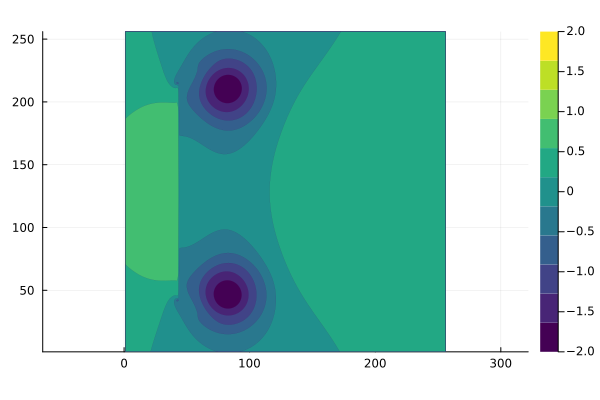
\includegraphics[trim={4cm 1.5cm 5cm 7cm},clip,width=\textwidth]{tex/fig/Disk_biot_press_3.png}
    \end{subfigure}
    \caption{Flow around an initially stationary disk accelerated in a quiescent flow at three convective times, $t^*\in [1,2,3]$, using the Biot-Savart boundary conditions. The entire computational domain is shown. The top half shows 10 iso-contour of the vorticity, equally spaced in the interval $\omega L/U\in\pm20$. The bottom half shows the pressure field, with 10 iso-contour equally spaced in $p/\rho U^2\in\pm2$.}
    \label{fig:disk_flow_2}
\end{figure}


\begin{figure}
    \centering
    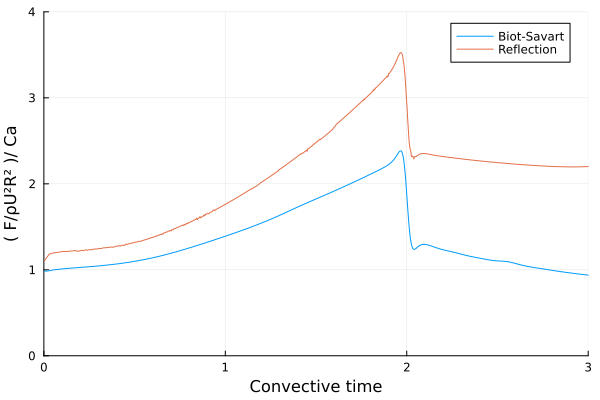
\includegraphics[width=0.5\textwidth]{tex//fig/Disk_256D_force.png}
    \caption{Instantaneous pressure force acting on the disk for the two different boundary conditions. The convective time corresponds to the snapshots shown in Fig.~\ref{fig:disk_flow_1}-\ref{fig:disk_flow_2}.}
    \label{fig:disk_forces}
\end{figure}


\subsection{3D Flow around a square disk at $Re=125\,000$}

To demonstrate the ability of our method to deal with highly separated and turbulent vortex formation, we simulate the flow around a square plate of dimension $L\times L$, accelerated in the surface normal direction to a final Reynolds number $Re=125\,000$. We focus on the initial vortex formation and position the plate at the center of a domain of size $2L\times2L\times2L$. For $t^*<6$, vortices typically stay attached to the body and only separate and travel downstream later, allowing us to use our Biot-Savart boundary conditions for this build-up phase. 

\begin{figure}
    \centering
    \begin{subfigure}{.33\textwidth}
        \centering
        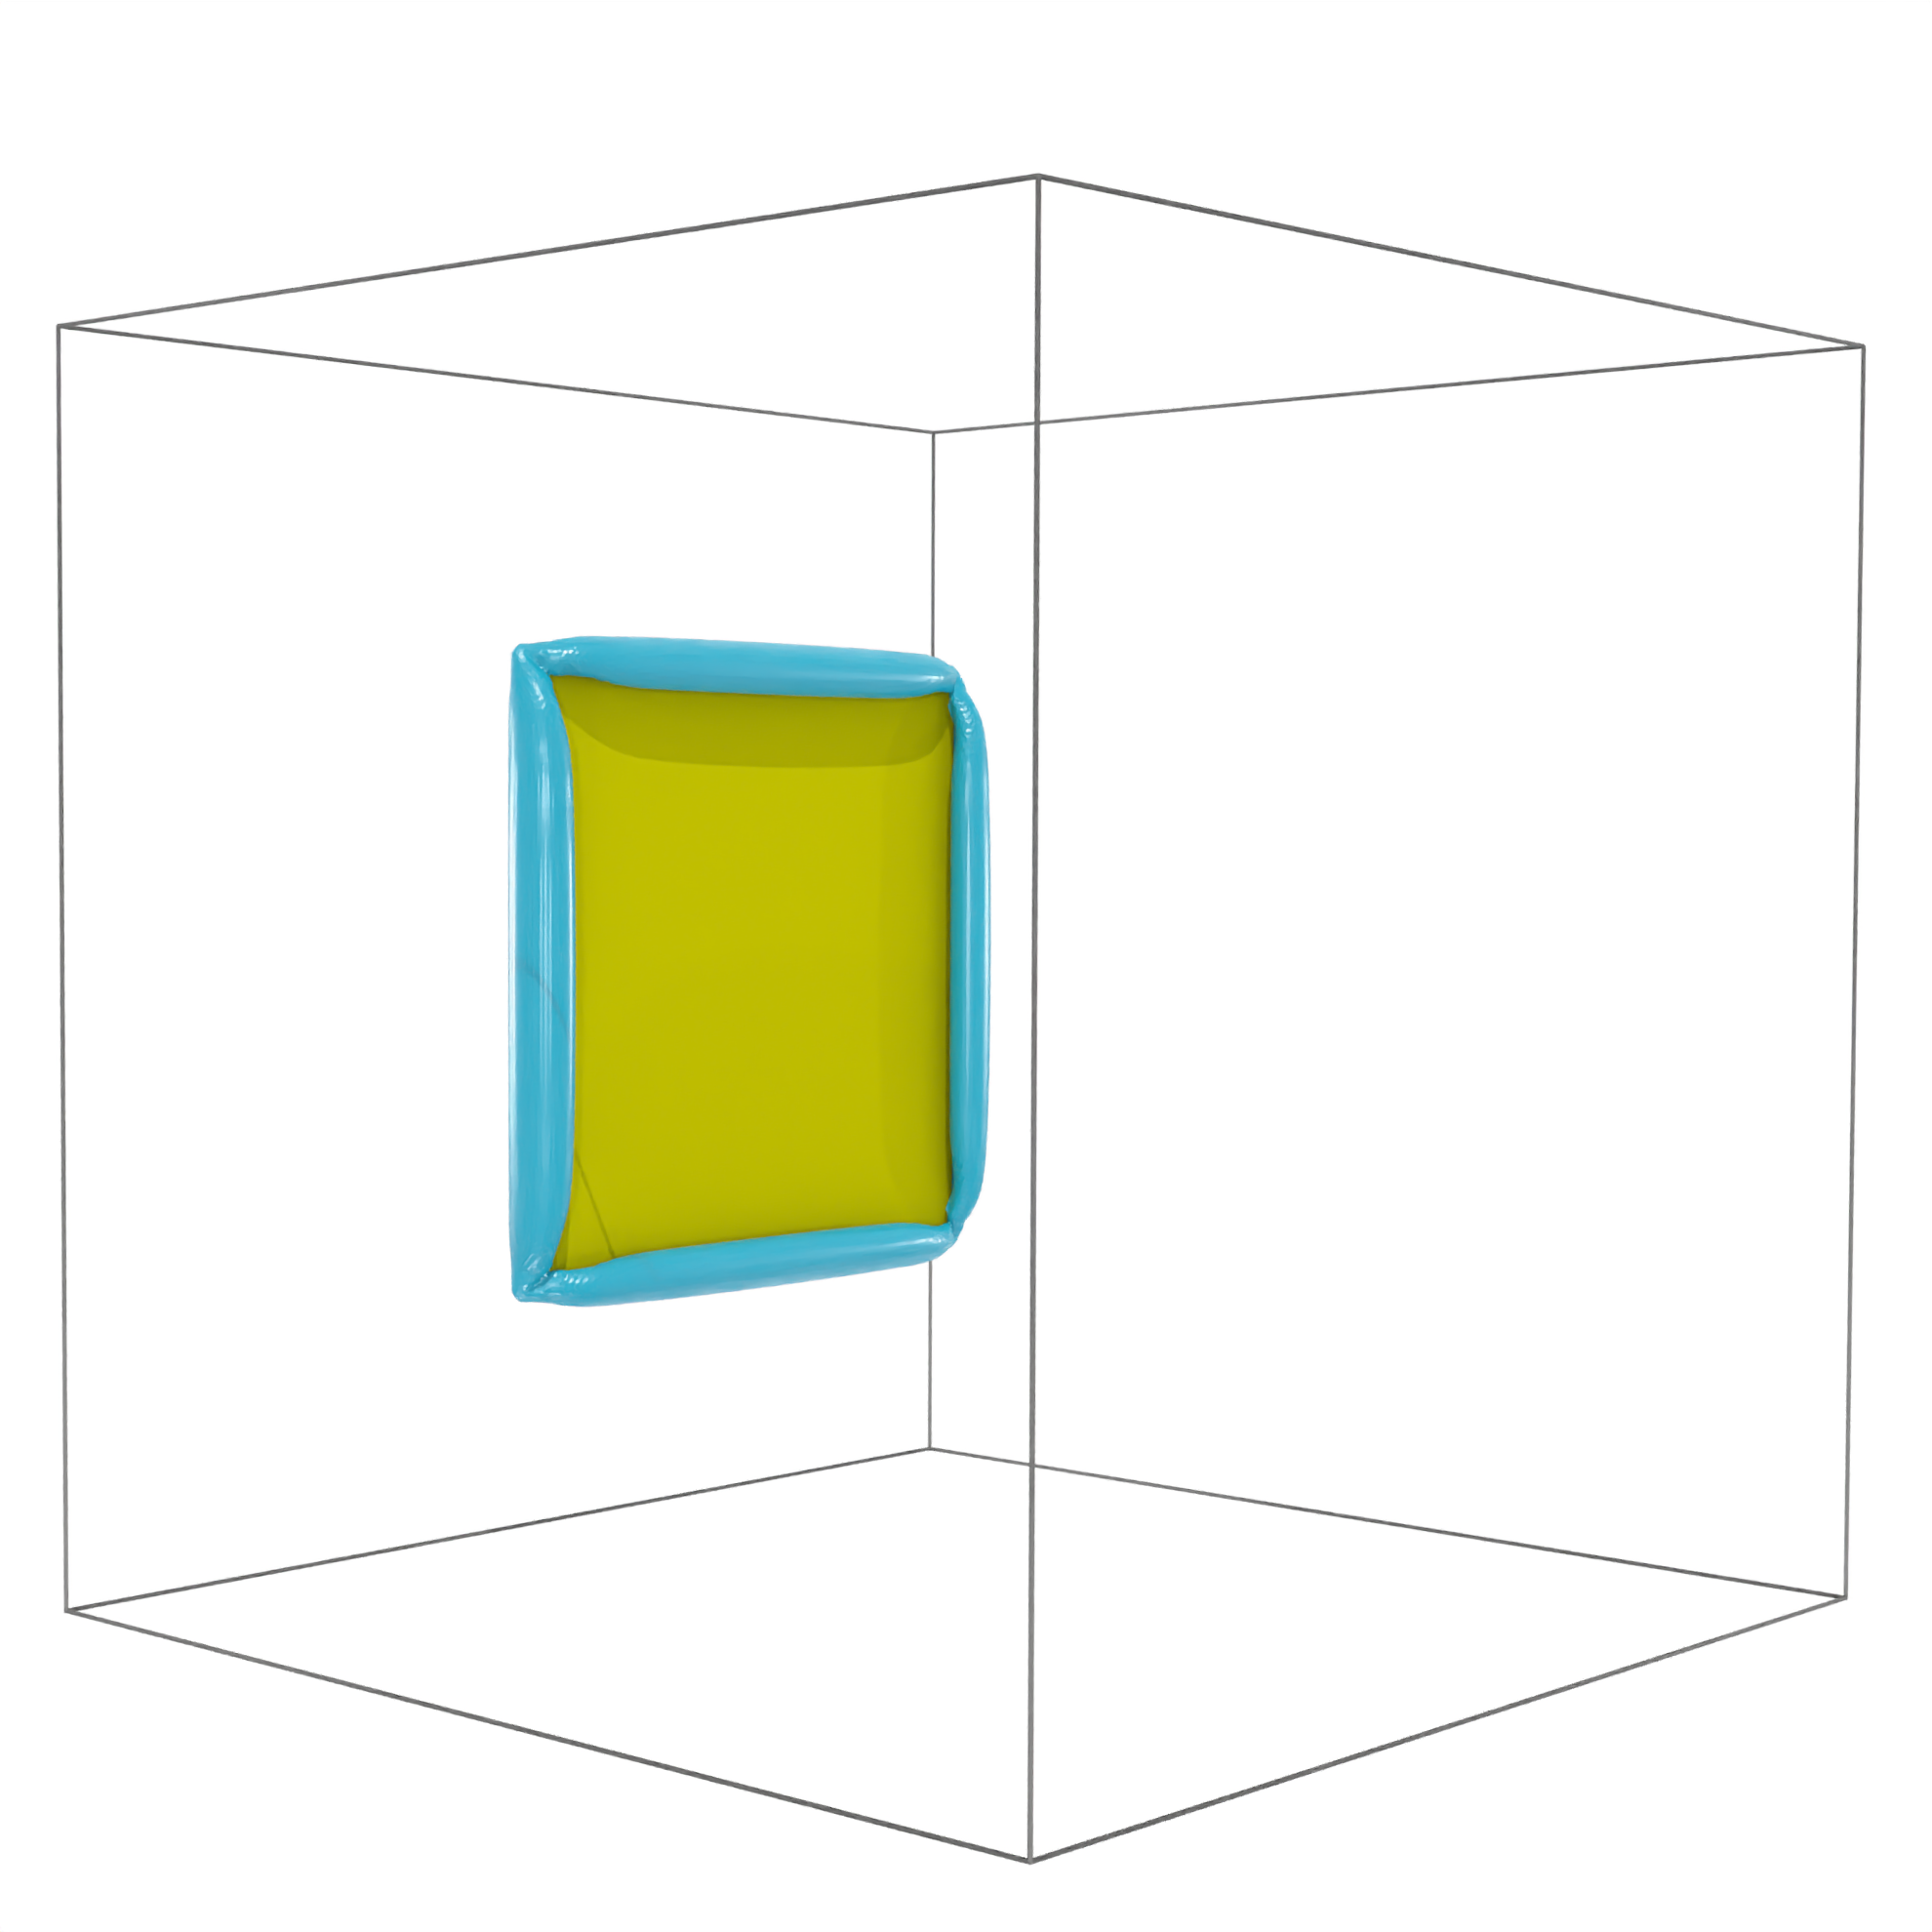
\includegraphics[width=\textwidth]{tex/fig/disk_high_re_2.png}
    \end{subfigure}%
    \begin{subfigure}{.33\textwidth}
        \centering
        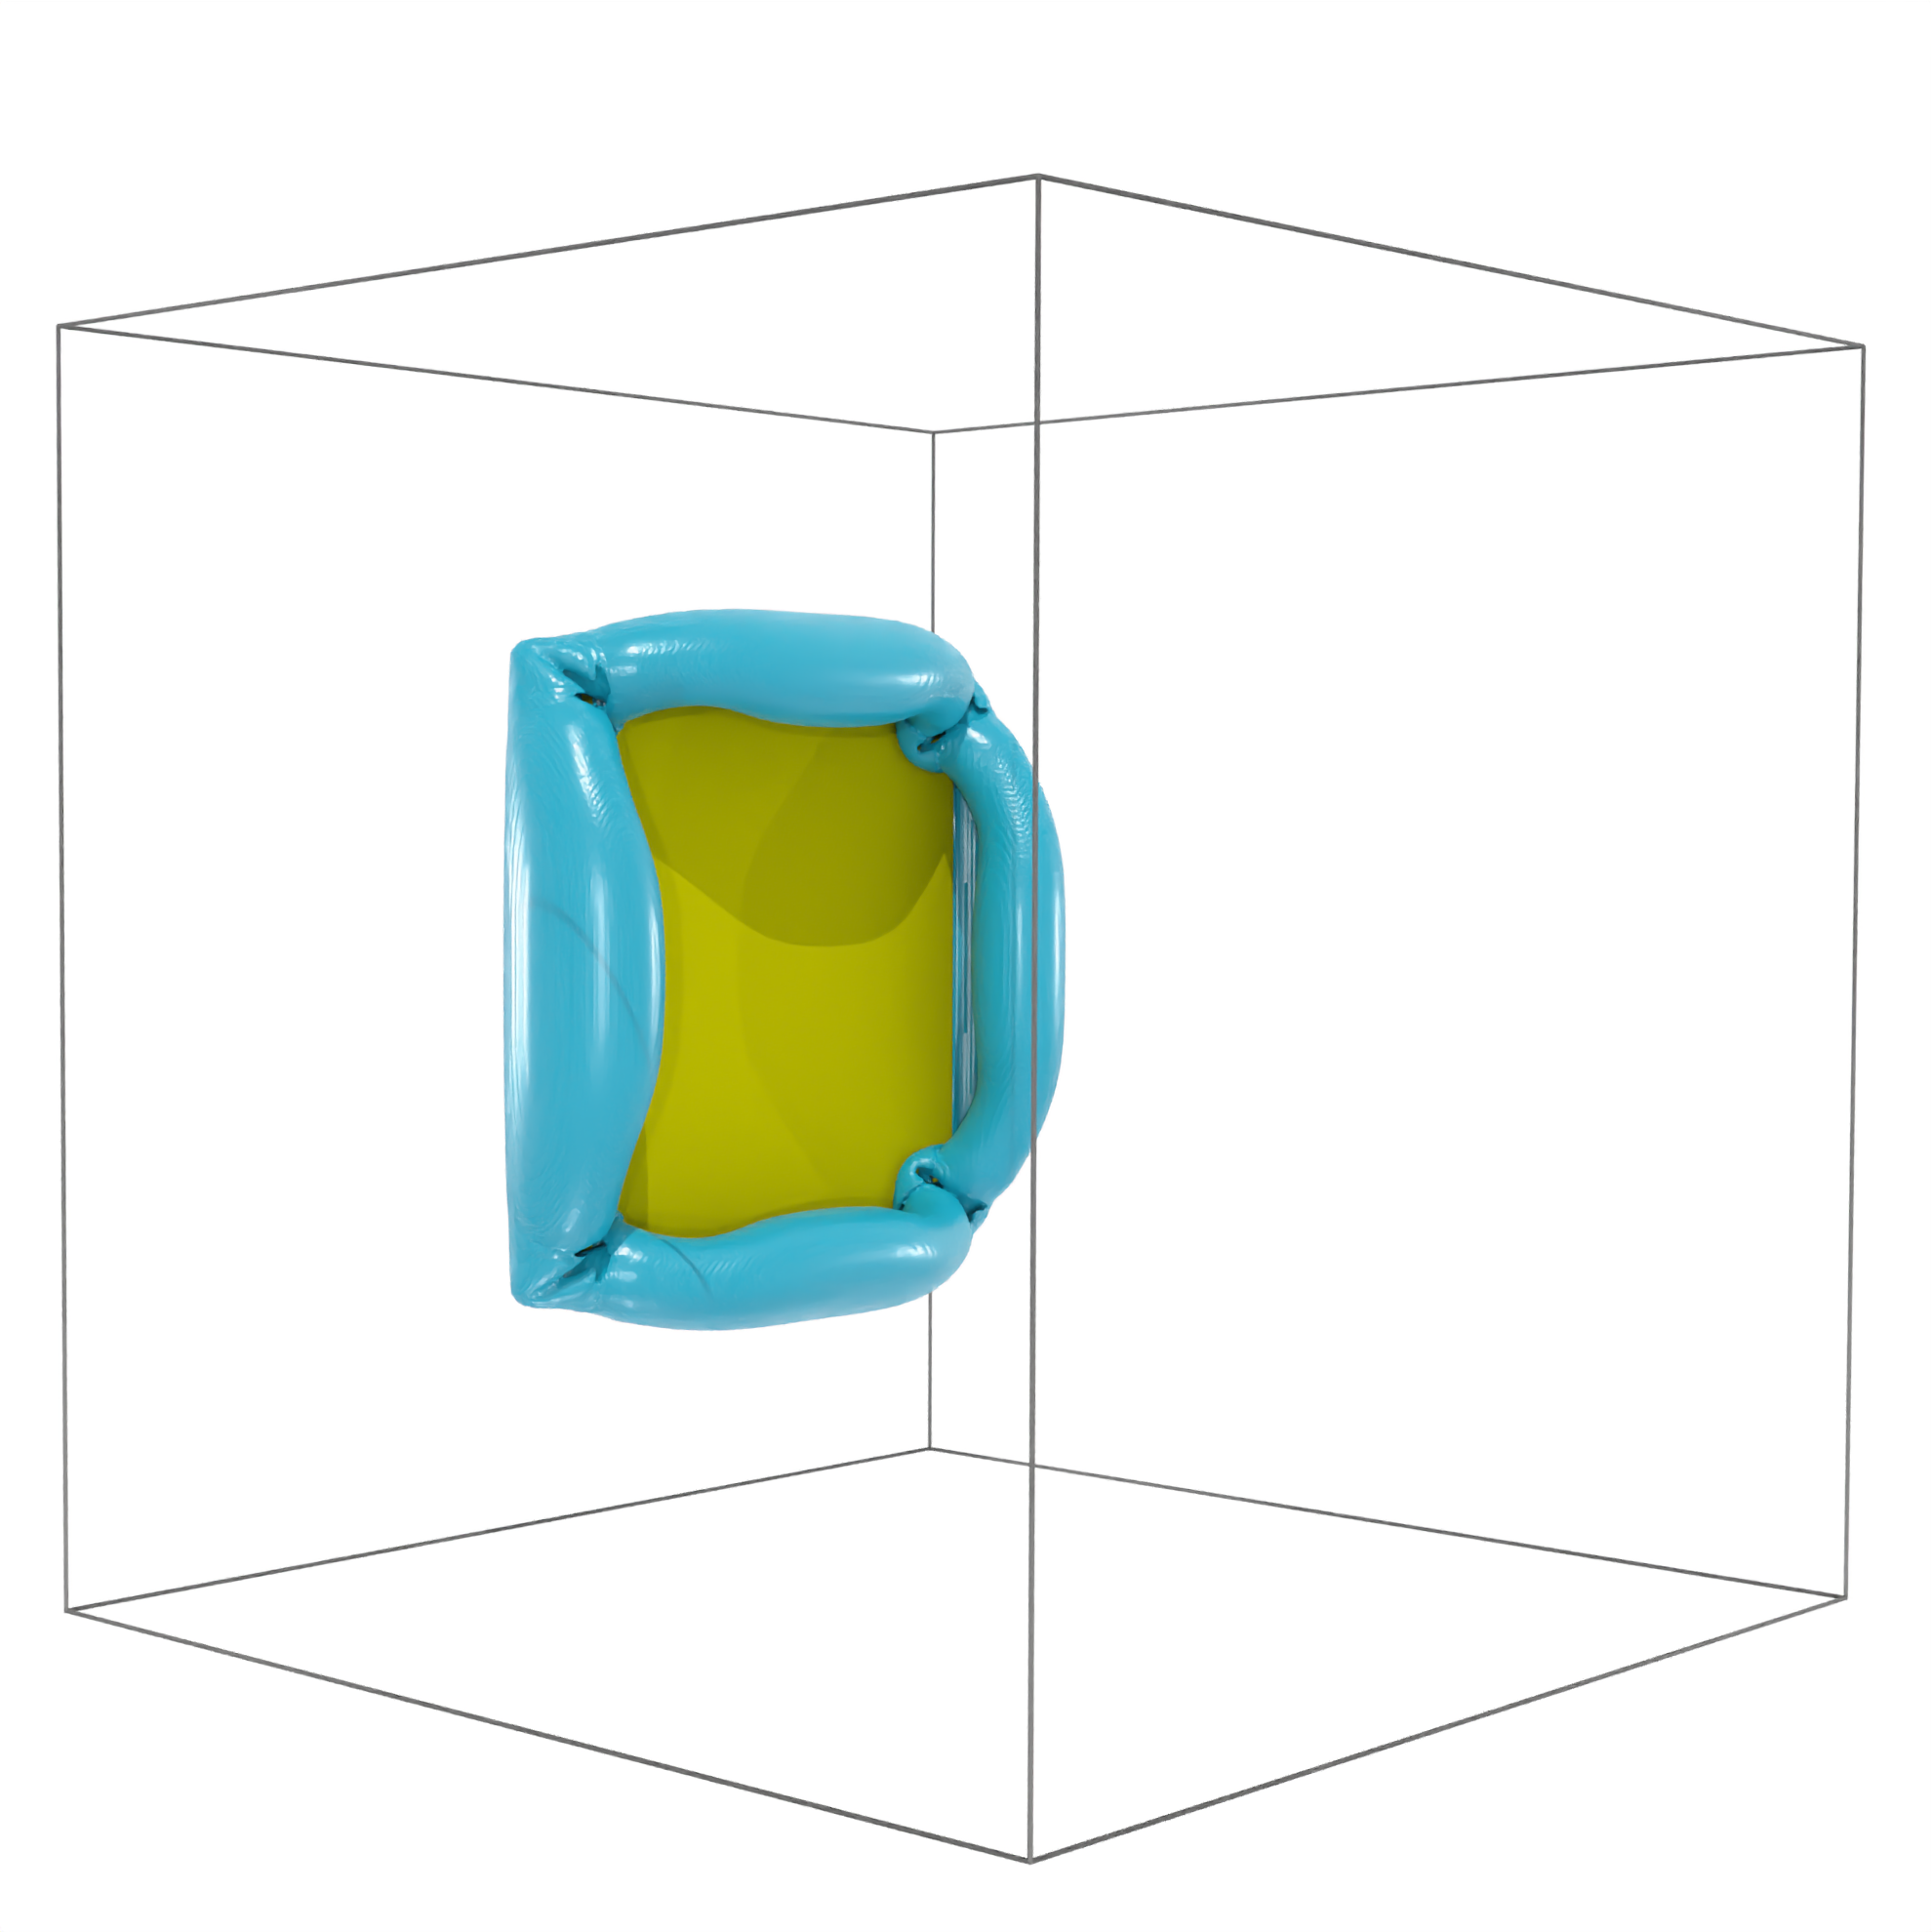
\includegraphics[width=\textwidth]{tex/fig/disk_high_re_3.png}
    \end{subfigure}%
    \begin{subfigure}{.33\textwidth}
        \centering
        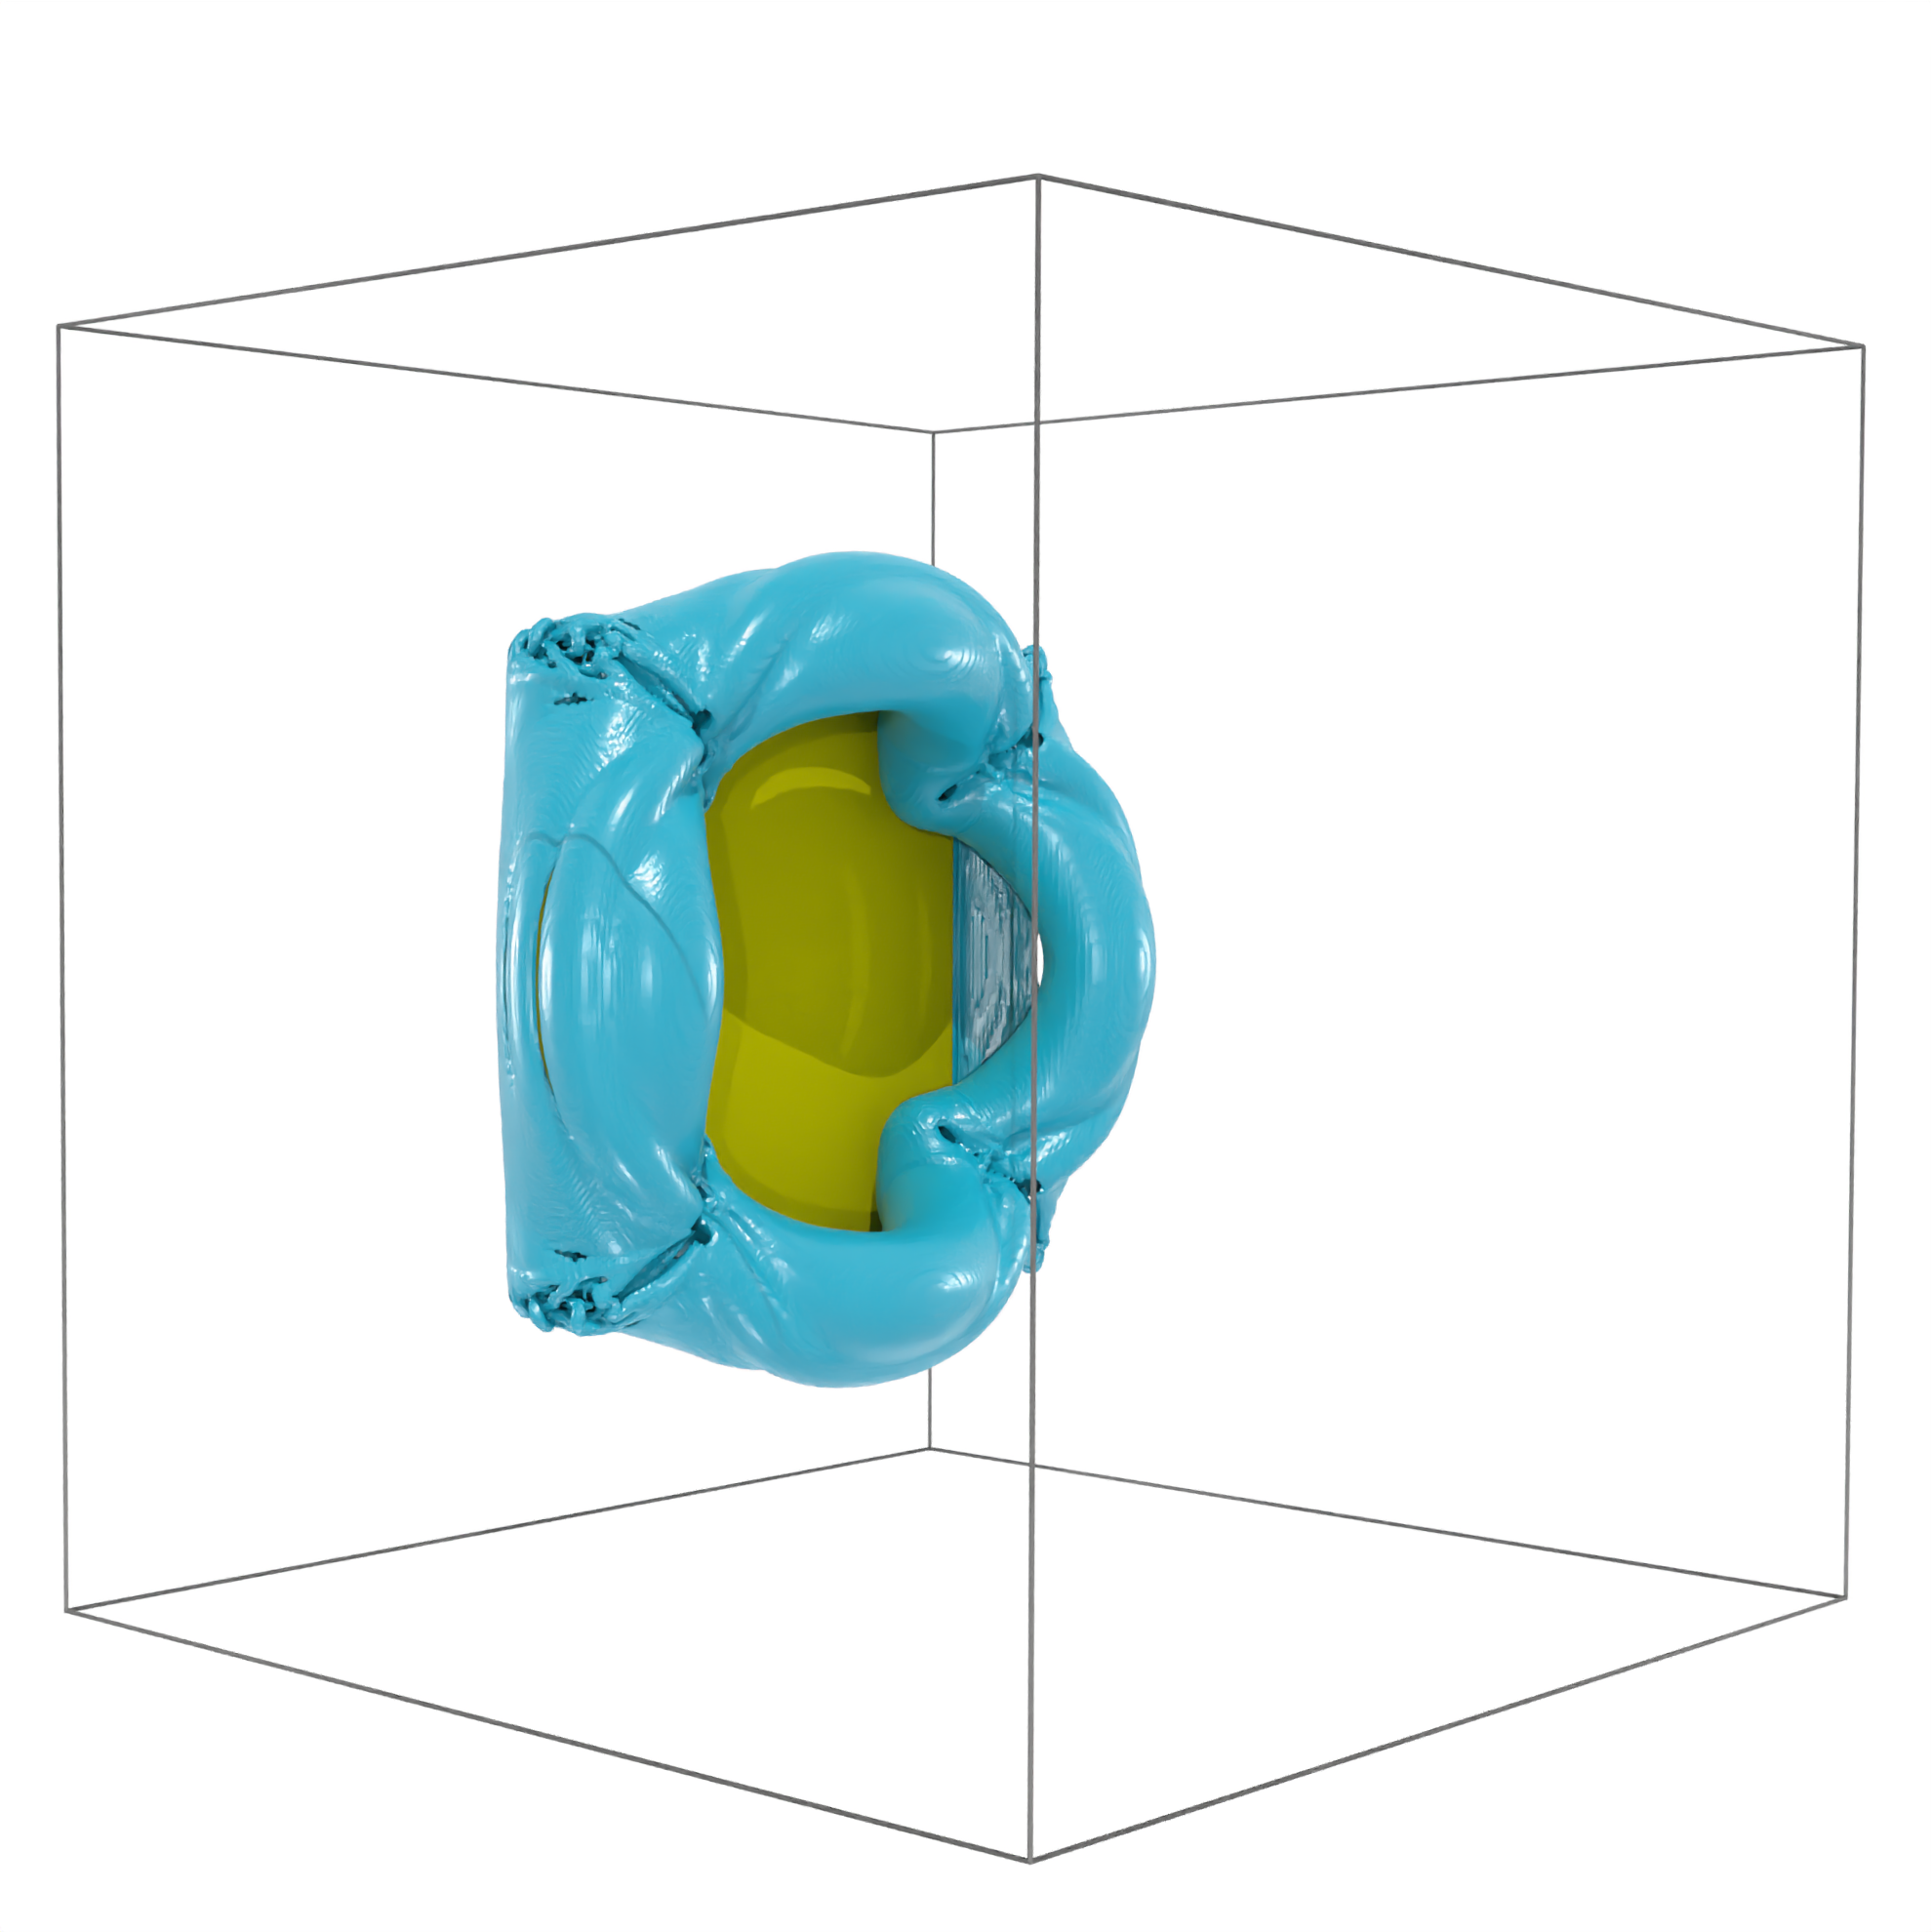
\includegraphics[width=\textwidth]{tex/fig/disk_high_re_4.png}
    \end{subfigure}
    \begin{subfigure}{.33\textwidth}
        \centering
        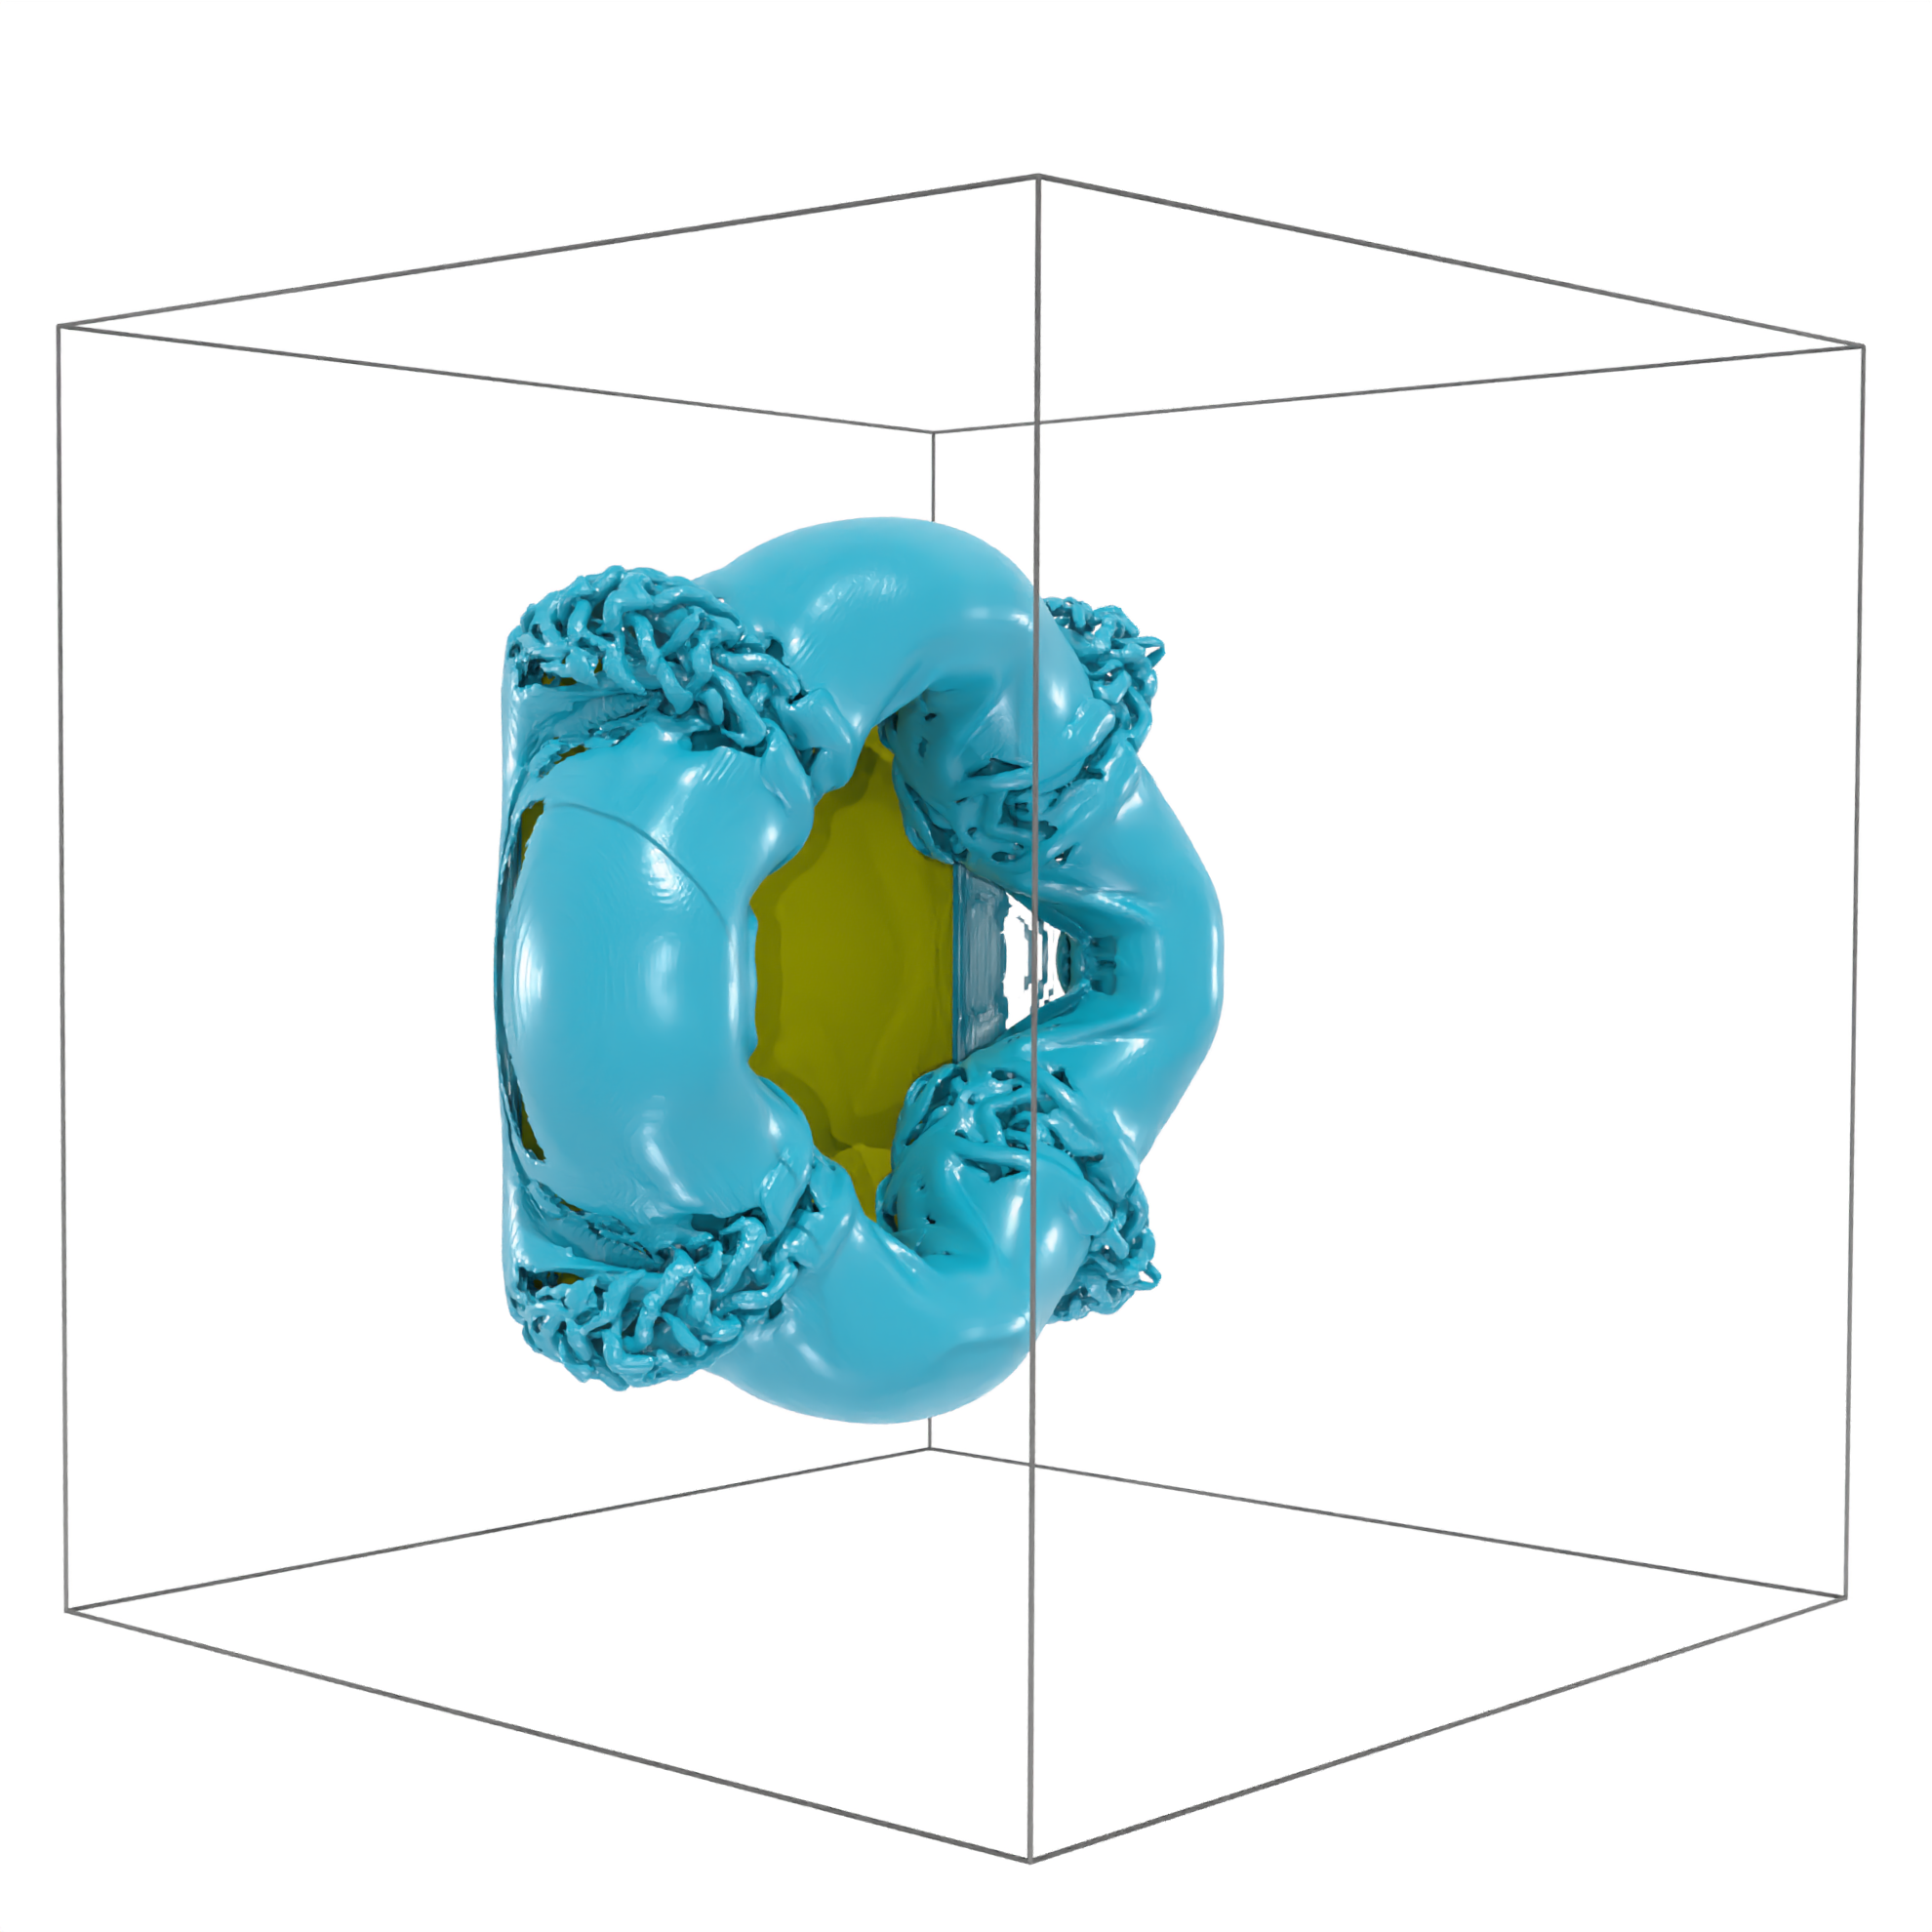
\includegraphics[width=\textwidth]{tex/fig/disk_high_re_5.png}
    \end{subfigure}%
    \begin{subfigure}{.33\textwidth}
        \centering
        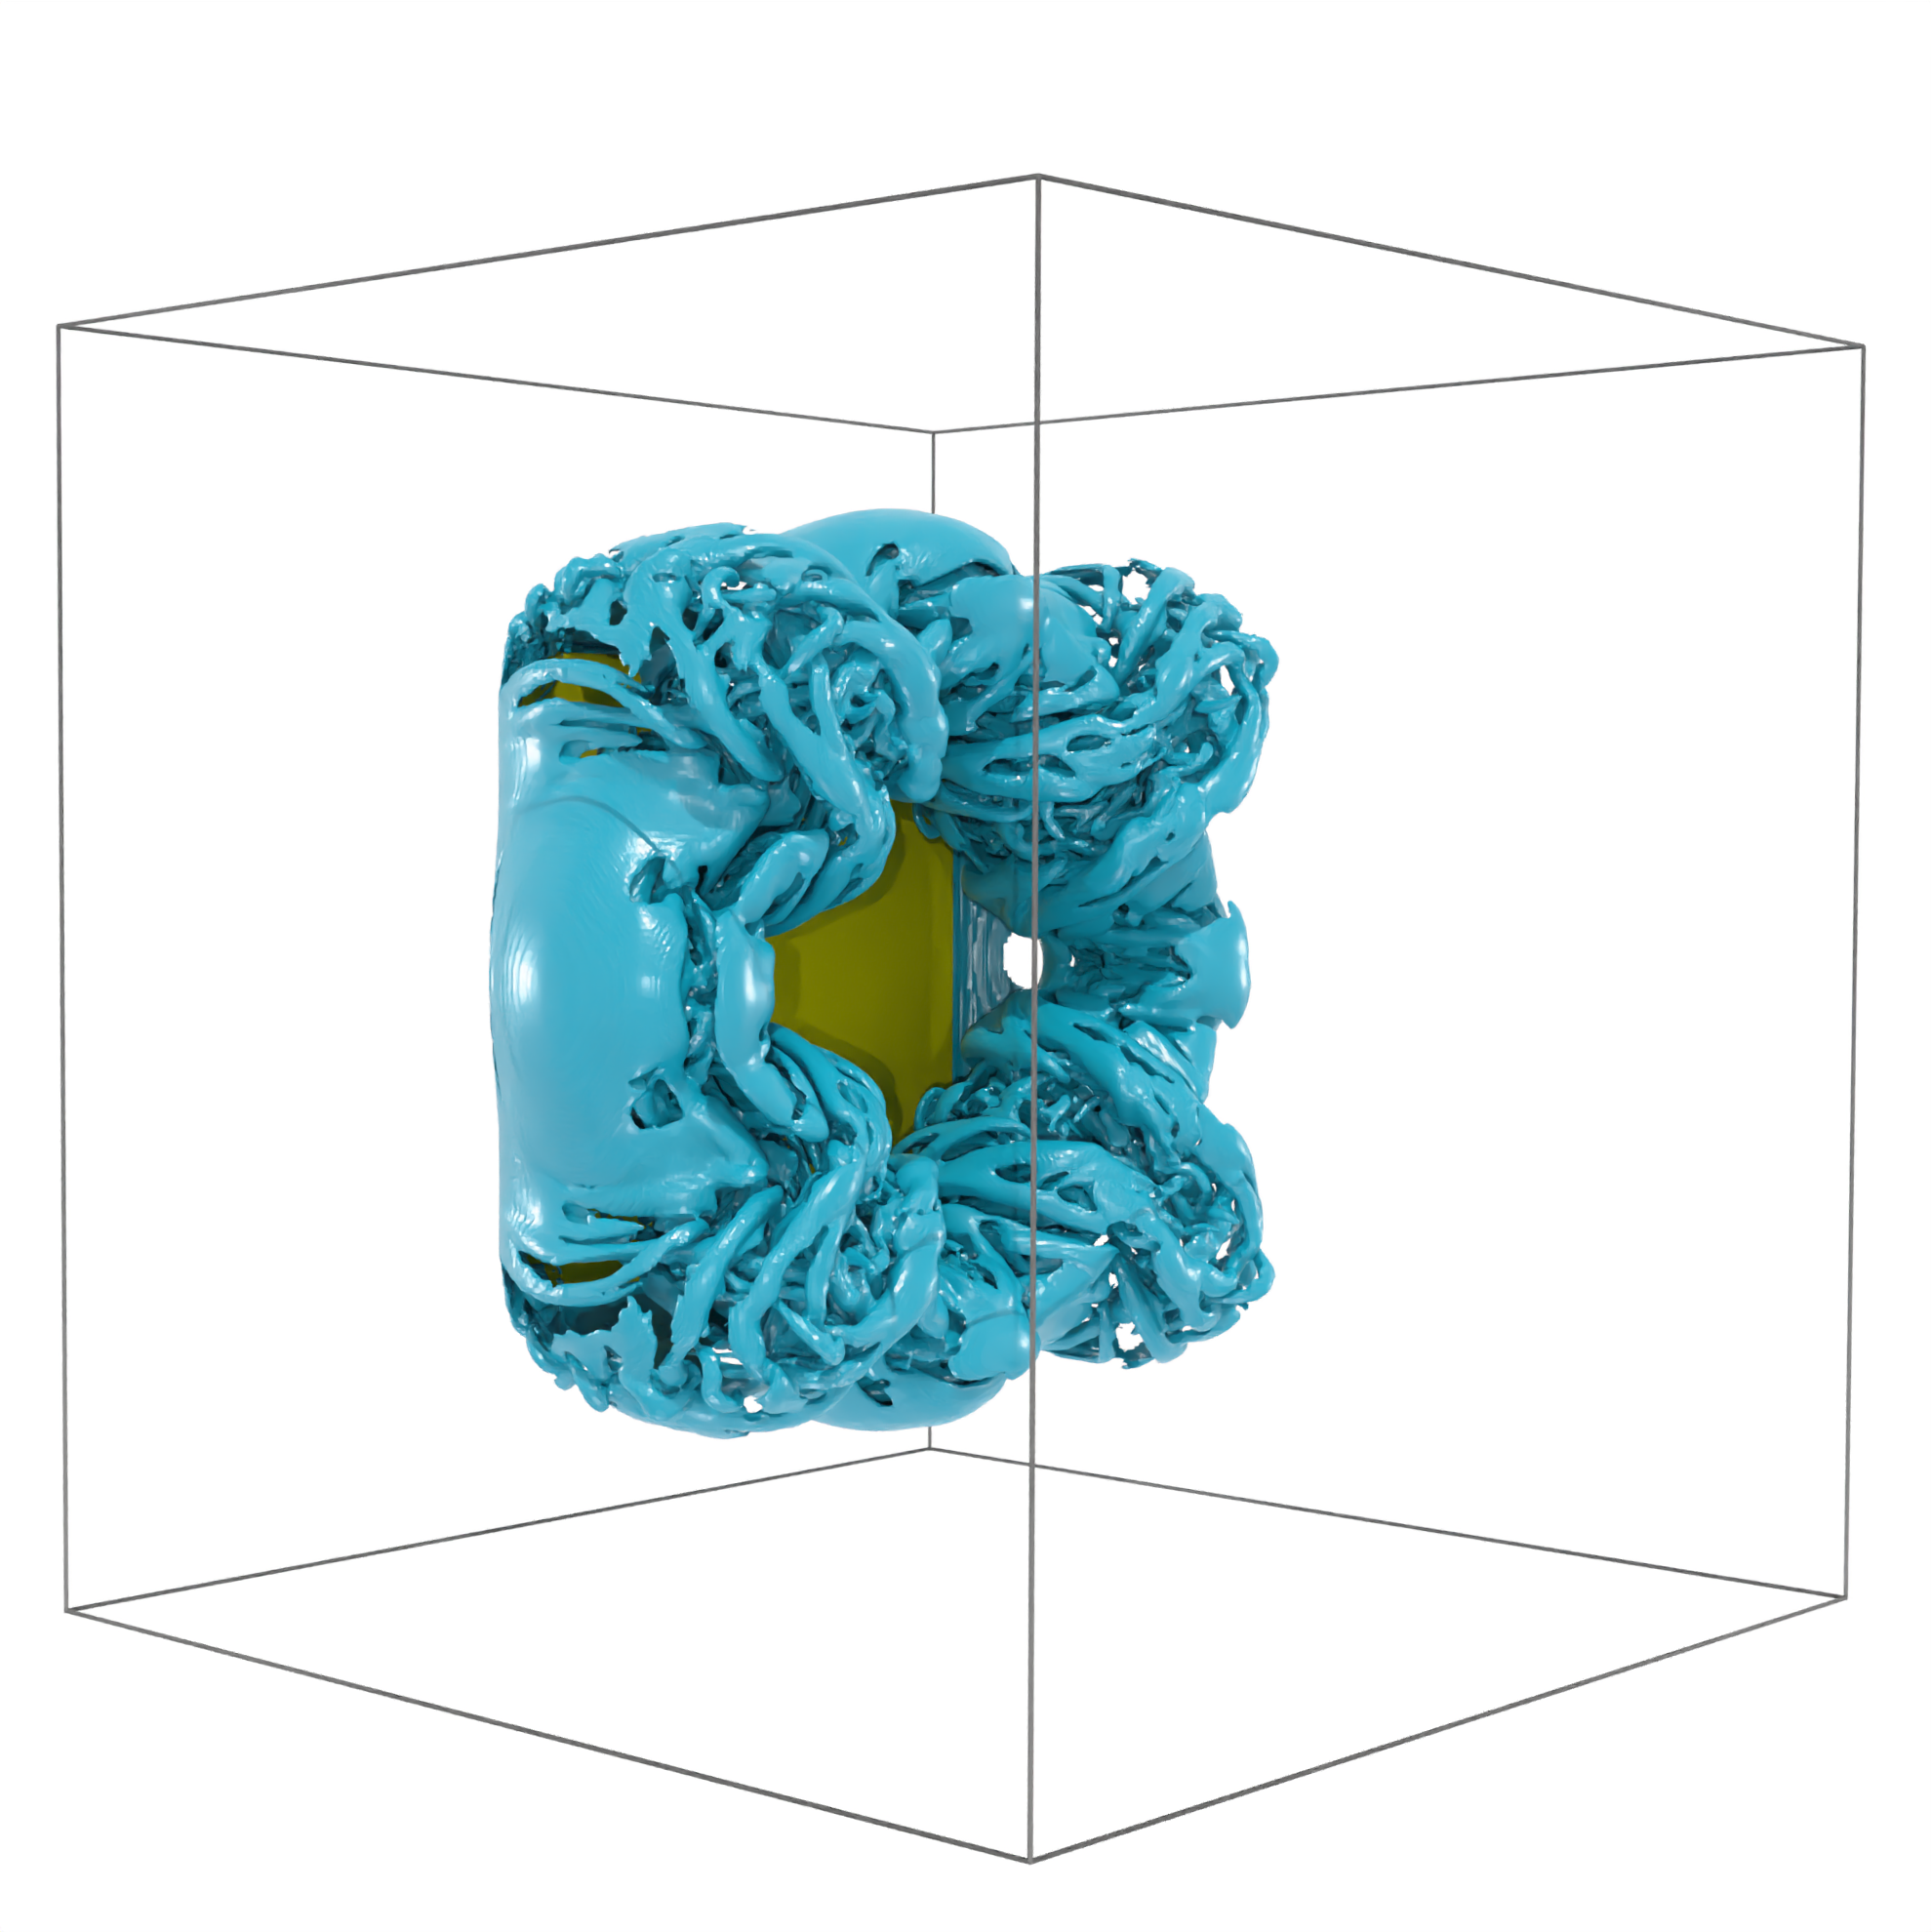
\includegraphics[width=\textwidth]{tex/fig/disk_high_re_6.png}
    \end{subfigure}%
    \begin{subfigure}{.33\textwidth}
        \centering
        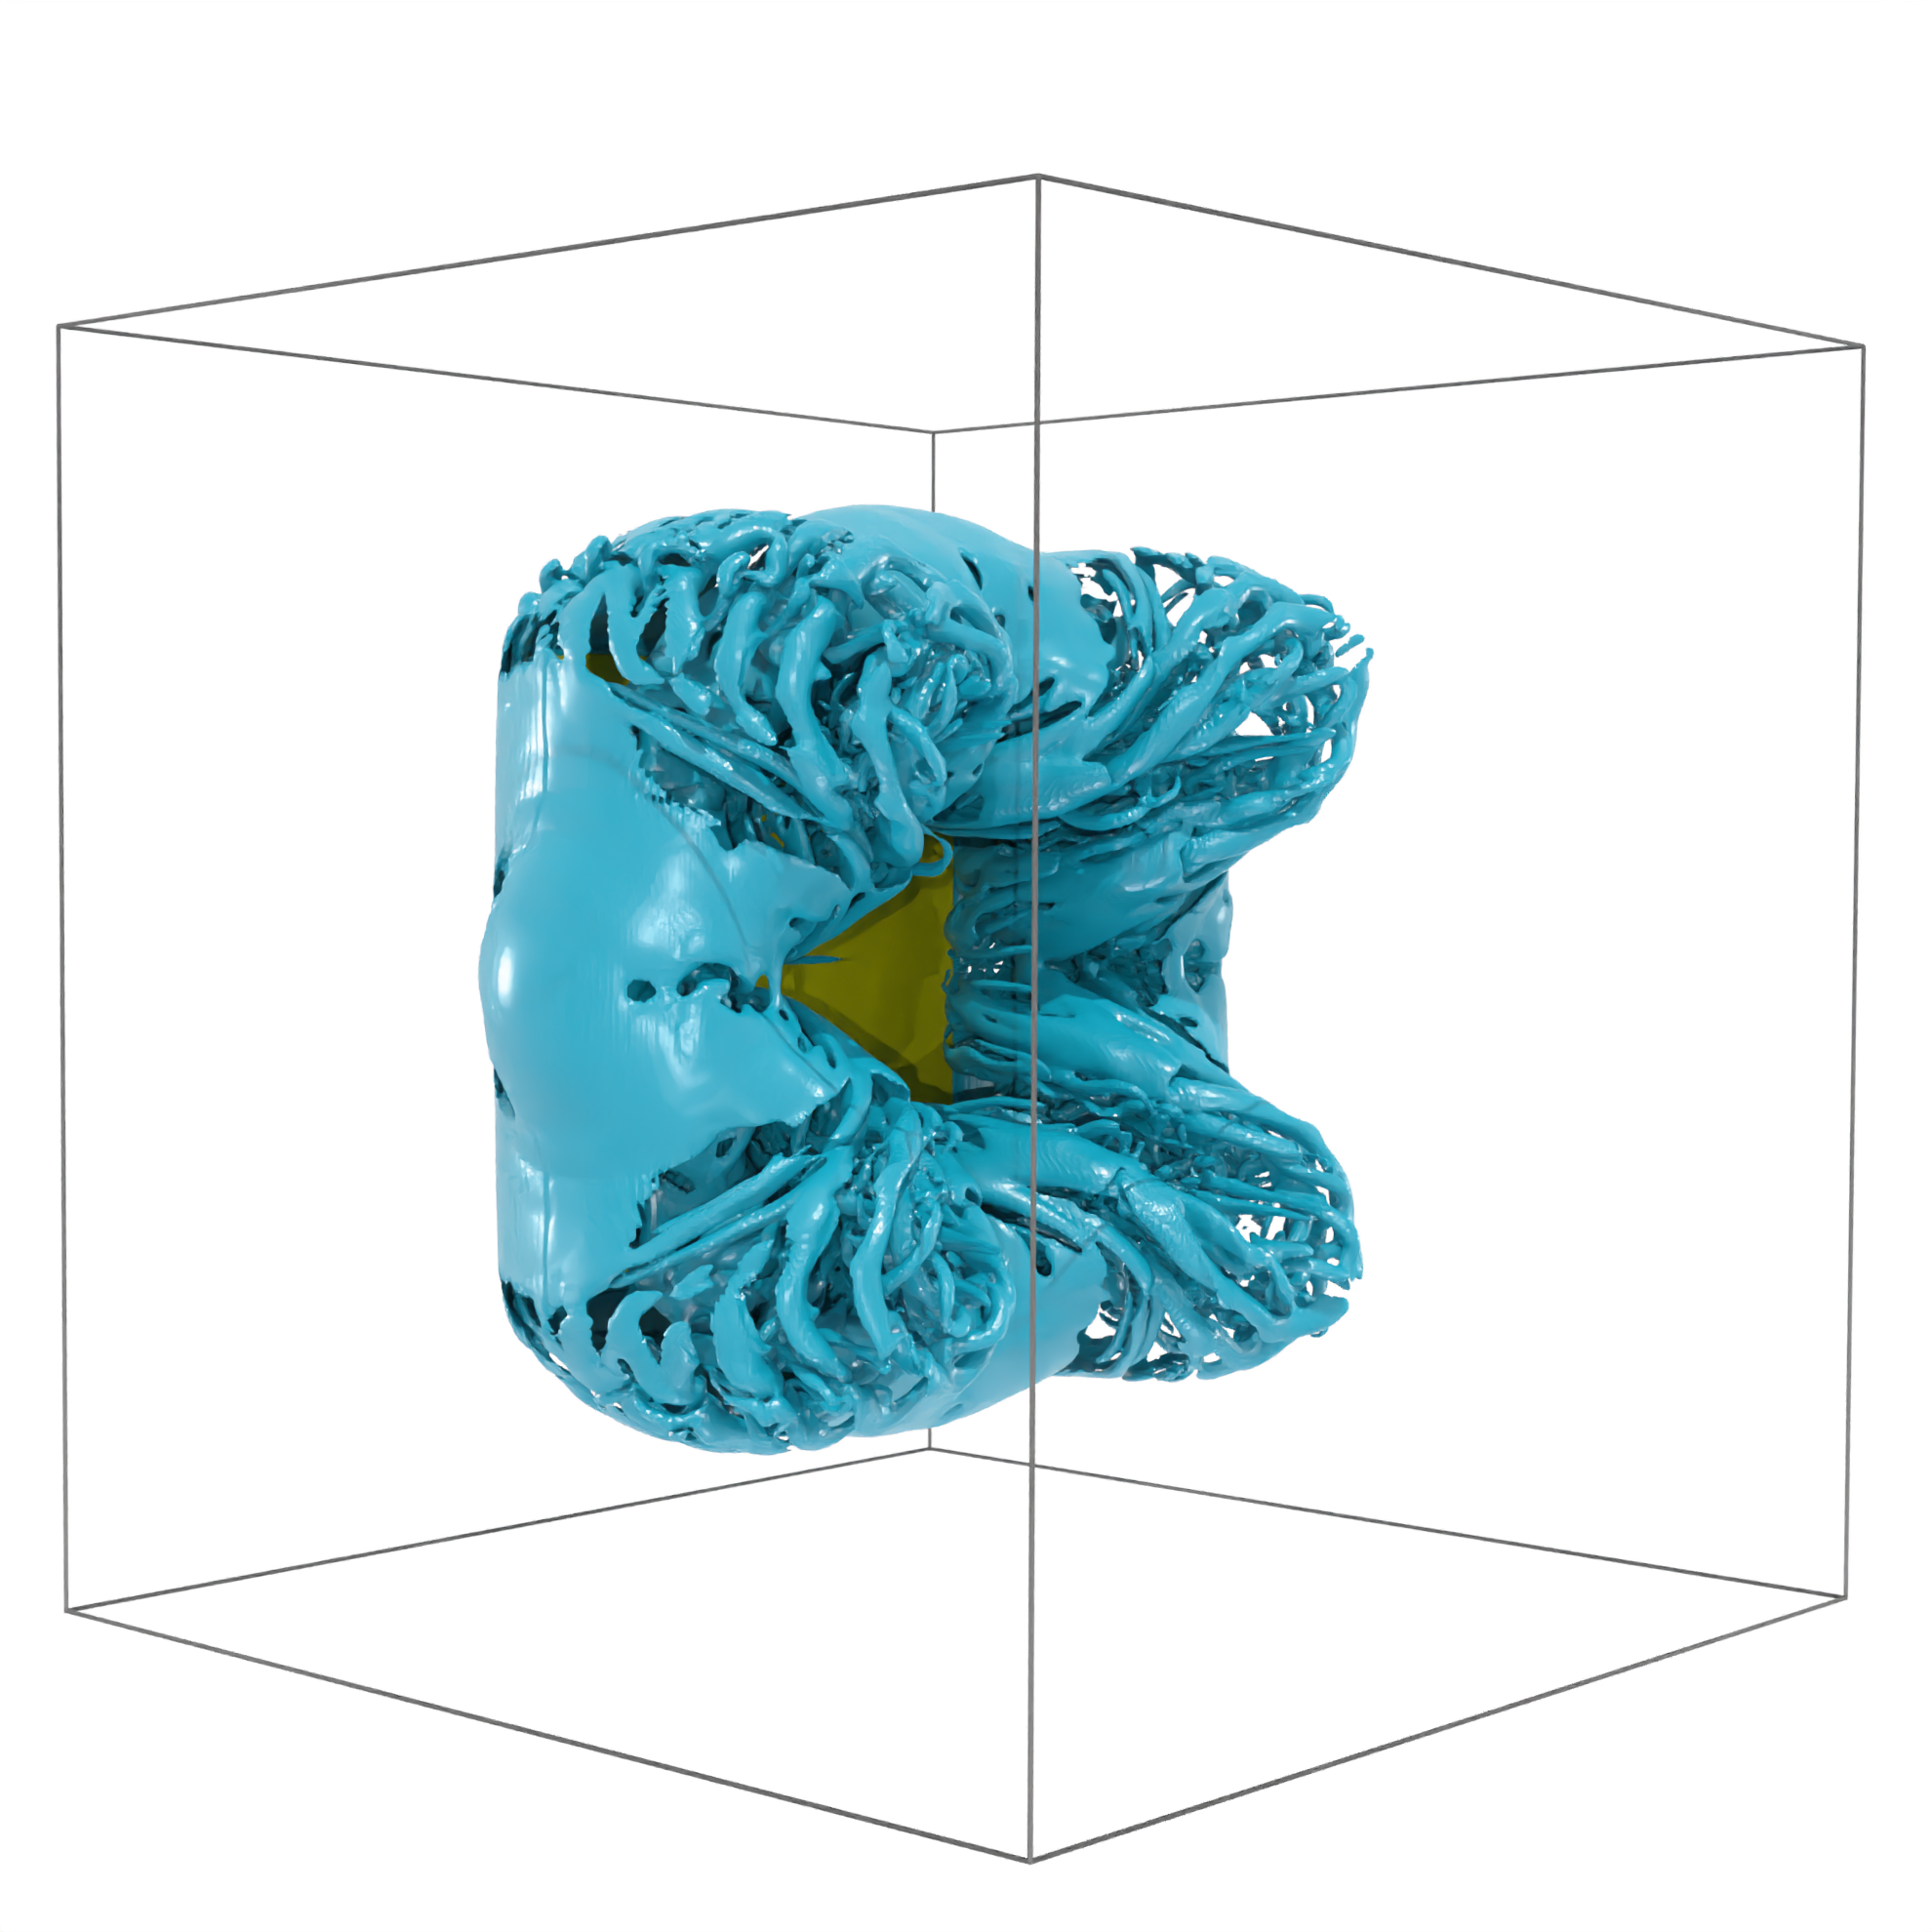
\includegraphics[width=\textwidth]{tex/fig/disk_high_re_7.png}
    \end{subfigure}
    \caption{Isocontour of $\lambda_2$-criterion $\lambda_2L^2/U^2=-2.7\times10^{-7}$ for the flow around an initially stationary square plate at $Re=125\,000$ accelerated from rest in a quiescent flow at 6 convective times, $t^*\in [1,2,3,4,5,6]$, using the Biot-Savart boundary conditions. The black frame represents the entire computational domain of size ($2L\times2L\times2L$). An animation of these still images in provided in the supplementary material.}
    \label{fig:disk_flow_3}
\end{figure}

Figure~\ref{fig:disk_flow_3} shows the vorticity generated by this accelerating body as six convective times $t^*\in[1,2,3,4,5,6]$. The vortices generated are shown via the $\lambda_2$-criterion \cite{JEong1995OnVortex}. The initial impulse generates a strong shear layer around the plate's edge that induces a strong vortex. Although the platform of the plate is square, this initial vortex rearrange itself into a shape resembling that of a vortex ring. After this initial vortex has traveled downstream, the plate's corner starts shedding smaller vortices that later trigger the breakdown of the start vortex. An animation of these still frames is provided in the supplementary material.

\section{Vortex-street applications}

Numerous examples of external flow violate our initial assumption that the vorticity is confined near the immersed body, far from the domain's boundary. We use two classical examples of vortex-street flows to investigate the effect of our short computational domain on flow history. First, the flow around a 2D cylinder at a Reynolds number $Re=200$, which results in the classical \emph{van K\`arm\`an} wake. Then, the reversed \emph{van K\`arm\`an} (or propulsive) wake generated by a heaving airfoil in a uniform flow at a range of Strouhal numbers.

\subsection{Flow around a 2D cylinder at $Re=200$}

We start our analysis with the flow behind a 2D circular cylinder of diameter $D$. The cylinder is immersed in a viscous fluid with free-stream velocity $U=(1,0)$. The viscosity is set such that the Reynolds number is $Re=\frac{UD}{\nu}=200$. We perform a domain study by varying the domain sizes from $5D\times3D$ up to $30D\times24D$ and, for each domain, compare the reflective and Biot-Savart boundary conditions.

Figure~\ref{fig:cylinder_force} shows the total drag force acting on the cylinder for the various domain sizes and boundary conditions. The different domain sizes and the Biot-Savart boundary conditions yield the best results with an excellent collapse of the drag forces, regardless of the domain size. Simulations performed with the Biot-Savart boundary conditions are insensitive to domain size. Reflective boundary conditions induce extremely large blockage effects for small domains and only slowly converge to the Biot-Savart boundary solution for significantly larger domains.

Additionaly, we compare the results obtained with a grid aligned with the mean flow direction to results obtained on a $7L\times 7L$ domain where the flow direction is $\vec{U}=(1/\sqrt{2},1/\sqrt{2})$ with the Biot-Savart boundary conditions. Results are also presented in Fig.~\ref{fig:cylinder_force} and are almost indistinguishable from the results using the aligned domain.

% We note here that the computational time for the smaller domain that uses the Biot-Savart boundary conditions is equivalent to that of \textbf{add computational time}. However, the convergence of the results with domain size is far superior.

In addition to the total drag forces acting on the cylinder, we look at the vortex shedding frequency in the wake. Here again, the Biot-Savart boundary conditions show an excellent collapse of the shedding frequency, which matches that of classical bluff body vortex shedding frequency of $St\sim 0.3$ \cite{}. The high blockage effect induced by the reflective boundary conditions induces fast flow around the cylinder, increasing the shedding frequency to higher values with reflective boundary conditions.

\begin{figure}
    \centering
    \begin{subfigure}{.5\textwidth}
        \centering
        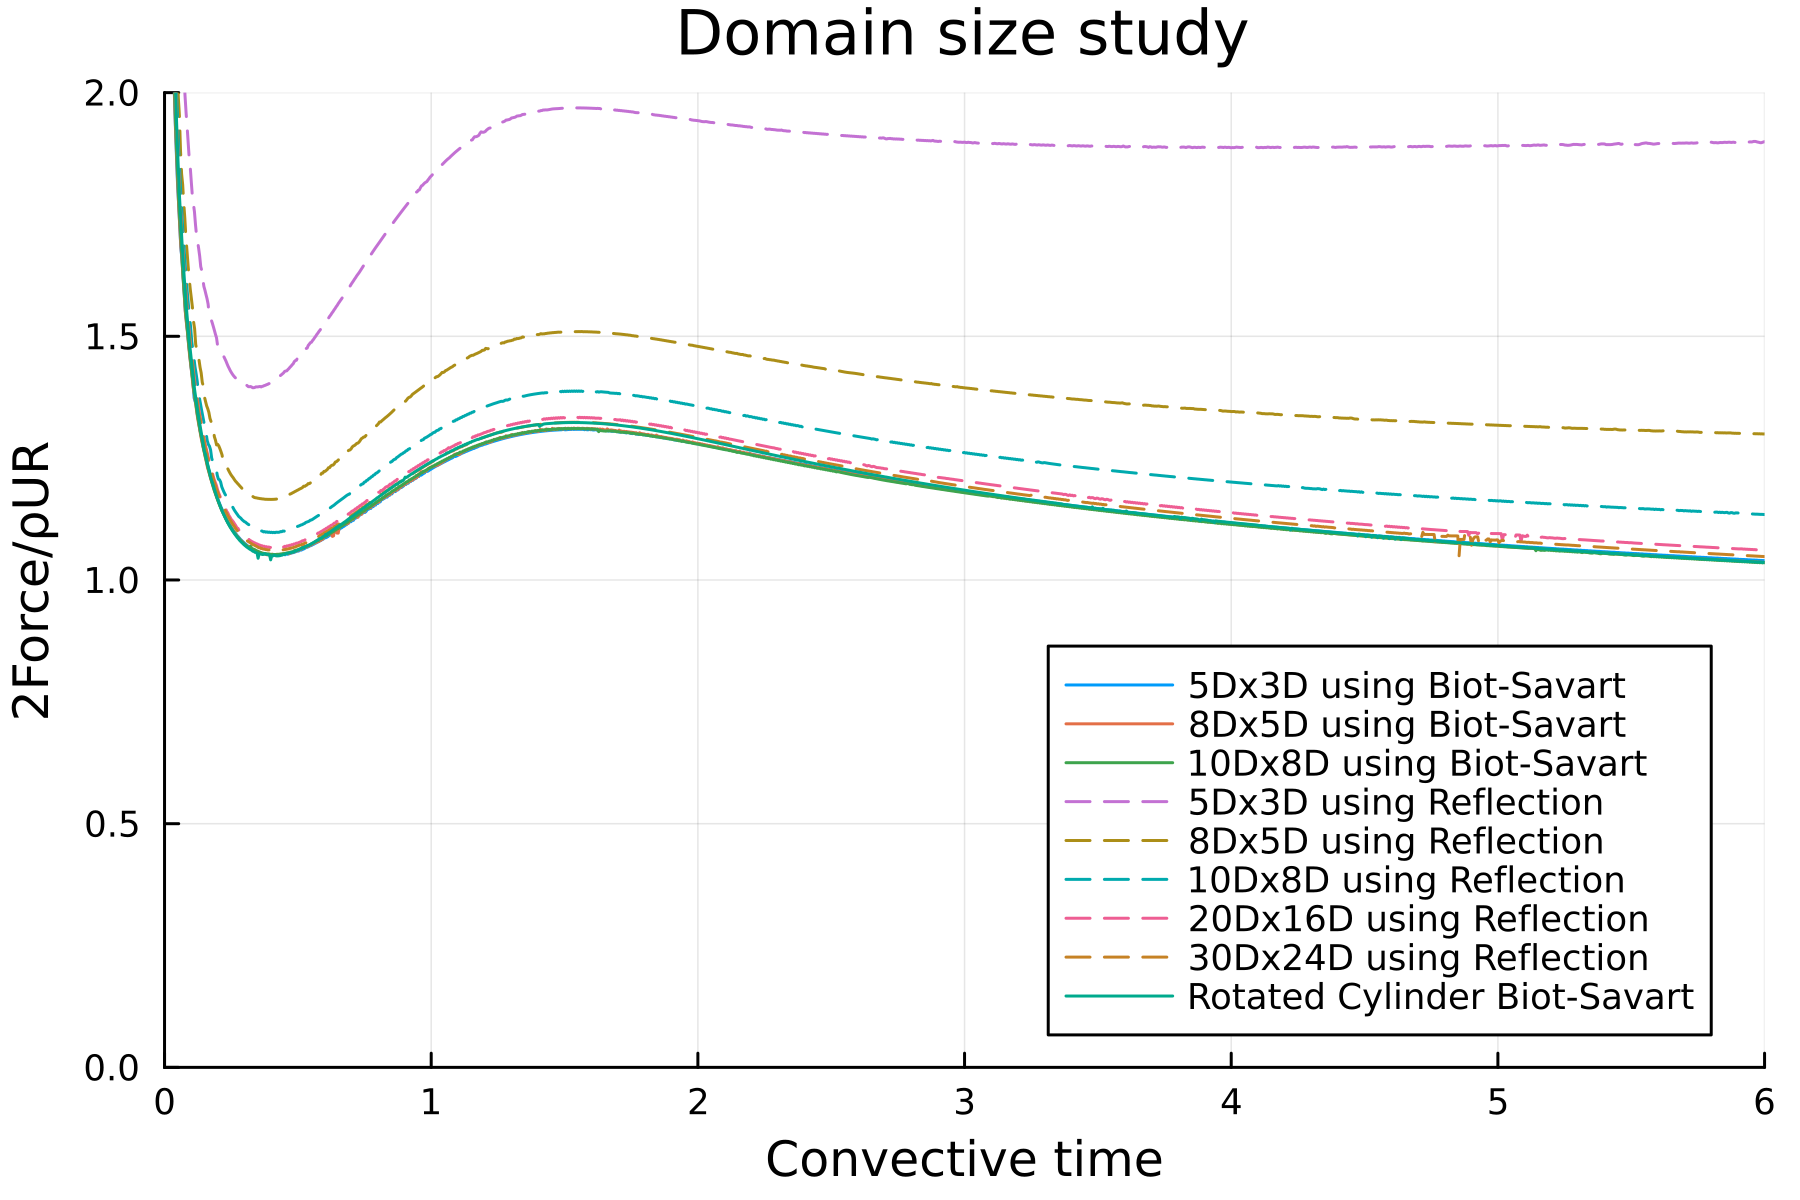
\includegraphics[width=\textwidth]{tex//fig/force.png}
    \end{subfigure}%
    \begin{subfigure}{.5\textwidth}
        \centering
        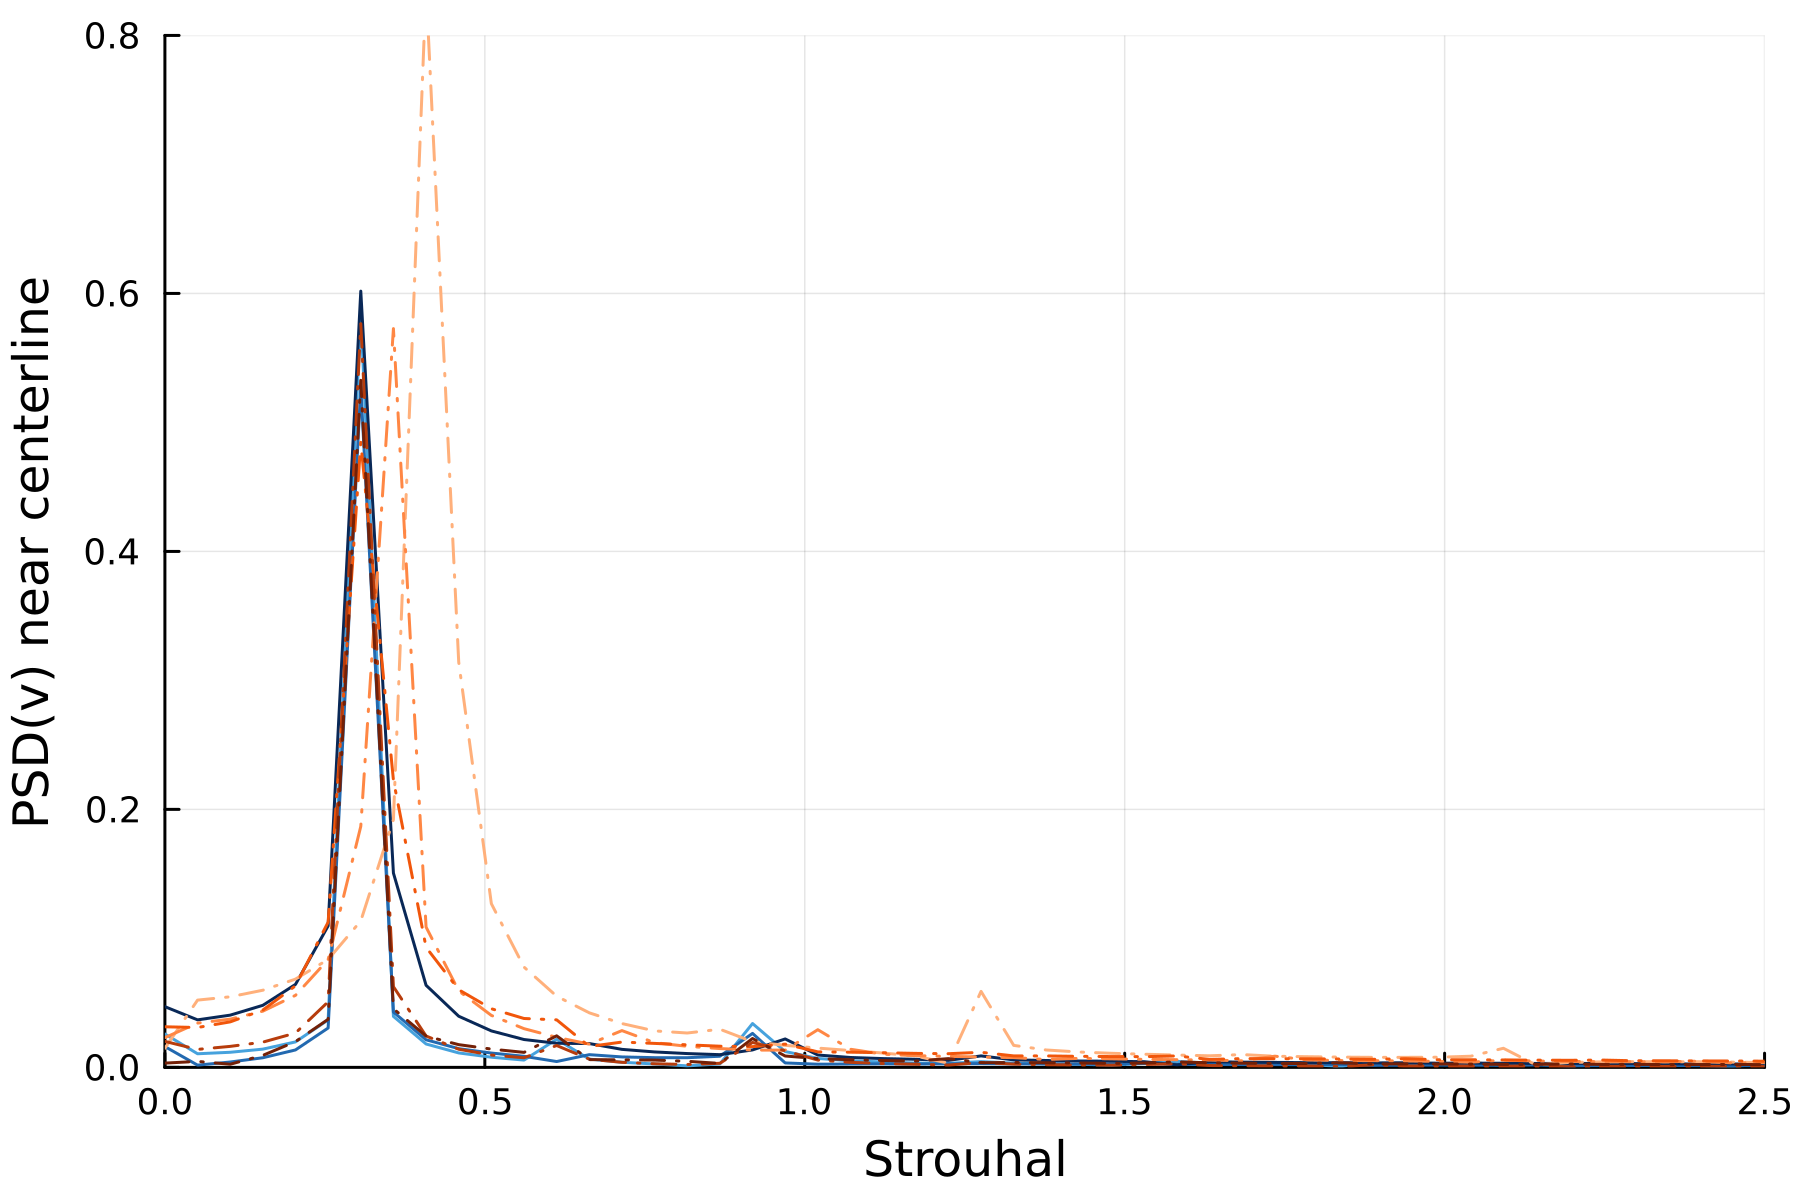
\includegraphics[width=\textwidth]{tex/fig/fft.png}
    \end{subfigure}%
    \caption{(left) Drag force acting on the circular cylinder at $Re=200$ for various combinations of boundary conditions and domain size. The rotated domain consists of a $4D\times4D$ domain, with the cylinder centered at $1.5D\times1.5D$ and a free stream velocity of $\vec{U}=(1/\sqrt2,1/\sqrt2)$. (right) The frequency spectrum of the wake of the cylinder for the same combination of boundary conditions and domain size shows the classical shedding frequency at $St=0.3$.}
    \label{fig:cylinder_force}
\end{figure}

These results suggest that, for drag wakes at least, the wake history on the immersed body is very small. However, propulsive systems use thrust wakes where wake history is expected to be higher.

\subsection{Wake behind a heaving foil}

We continue our analysis with thrust wakes. We immerse a rigid foil of length $L$ moving with a linear velocity $\vec{U}=(U,0)$ in a viscous fluid. In addition to its steady forward speed, the foil undergoes a pure heave motion of amplitude $h_0$
\begin{equation}
    y(t) = h_0 \sin(2\pi f t)
\end{equation}
where $h_0/L=0.5$ is the non-dimensional amplitude, and the frequency is $f = St\,U/h_0$. For Strouhal number $St<0.5$, the airfoil generates thrust, and almost no net lift, and for $St>0.6$, the wake generated by this flapping foil is strongly asymmetric and generates a significant net lift force. We perform simulations of this system for a range of Strouhal numbers and compare the mean lift force and wake obtained on a large domain ($30L\times20L$) with standard reflective boundary conditions to the ones obtained on two different domains of size ($6L\times4L$) and ($12L\times8L$) that use the Biot-Savart boundary conditions. We simulate the flow around this heaving airfoil for 100 convective times to ensure that the wake stabilizes, and we gather pressure and viscous forces for the last 20 convective times. Mean lift forces are obtained by time-averaging these forces over the past 20 convective times.

For $St<0.5$, we observe almost no difference between the different boundary conditions and domain sizes. The wake is symmetric, and the airfoil produces zero mean lift forces; see Fig.~\ref{fig:deflected_wake_2}. For $St\ge 0.5$ we start to observe wake deflection on the large domains with the reflective boundary condition.

\begin{figure}
    \centering
    \begin{subfigure}{.48\textwidth}
        \centering
        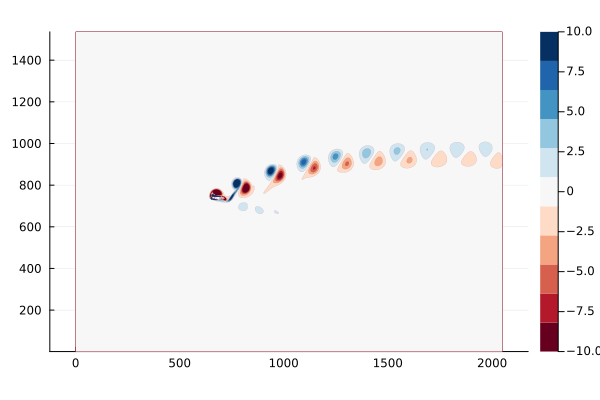
\includegraphics[trim={2.8cm 2cm 4cm 2cm},clip,width=\textwidth]{tex//fig/Deflected_wake_snap.png}
        \caption{Reflection ($30L\times20L$)}
    \end{subfigure}%
    \hspace{0.1cm}
    \begin{subfigure}{.48\textwidth}
        \centering
        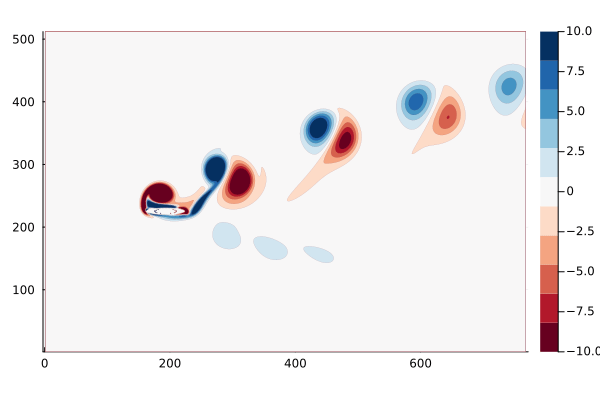
\includegraphics[trim={2.8cm 2cm 4cm 2cm},clip,width=\textwidth]{tex/fig/Deflected_wake_snap_small.png}
        \caption{Reflection ($30L\times20L$) - near wake}
    \end{subfigure}
    \begin{subfigure}{.48\textwidth}
        \centering
        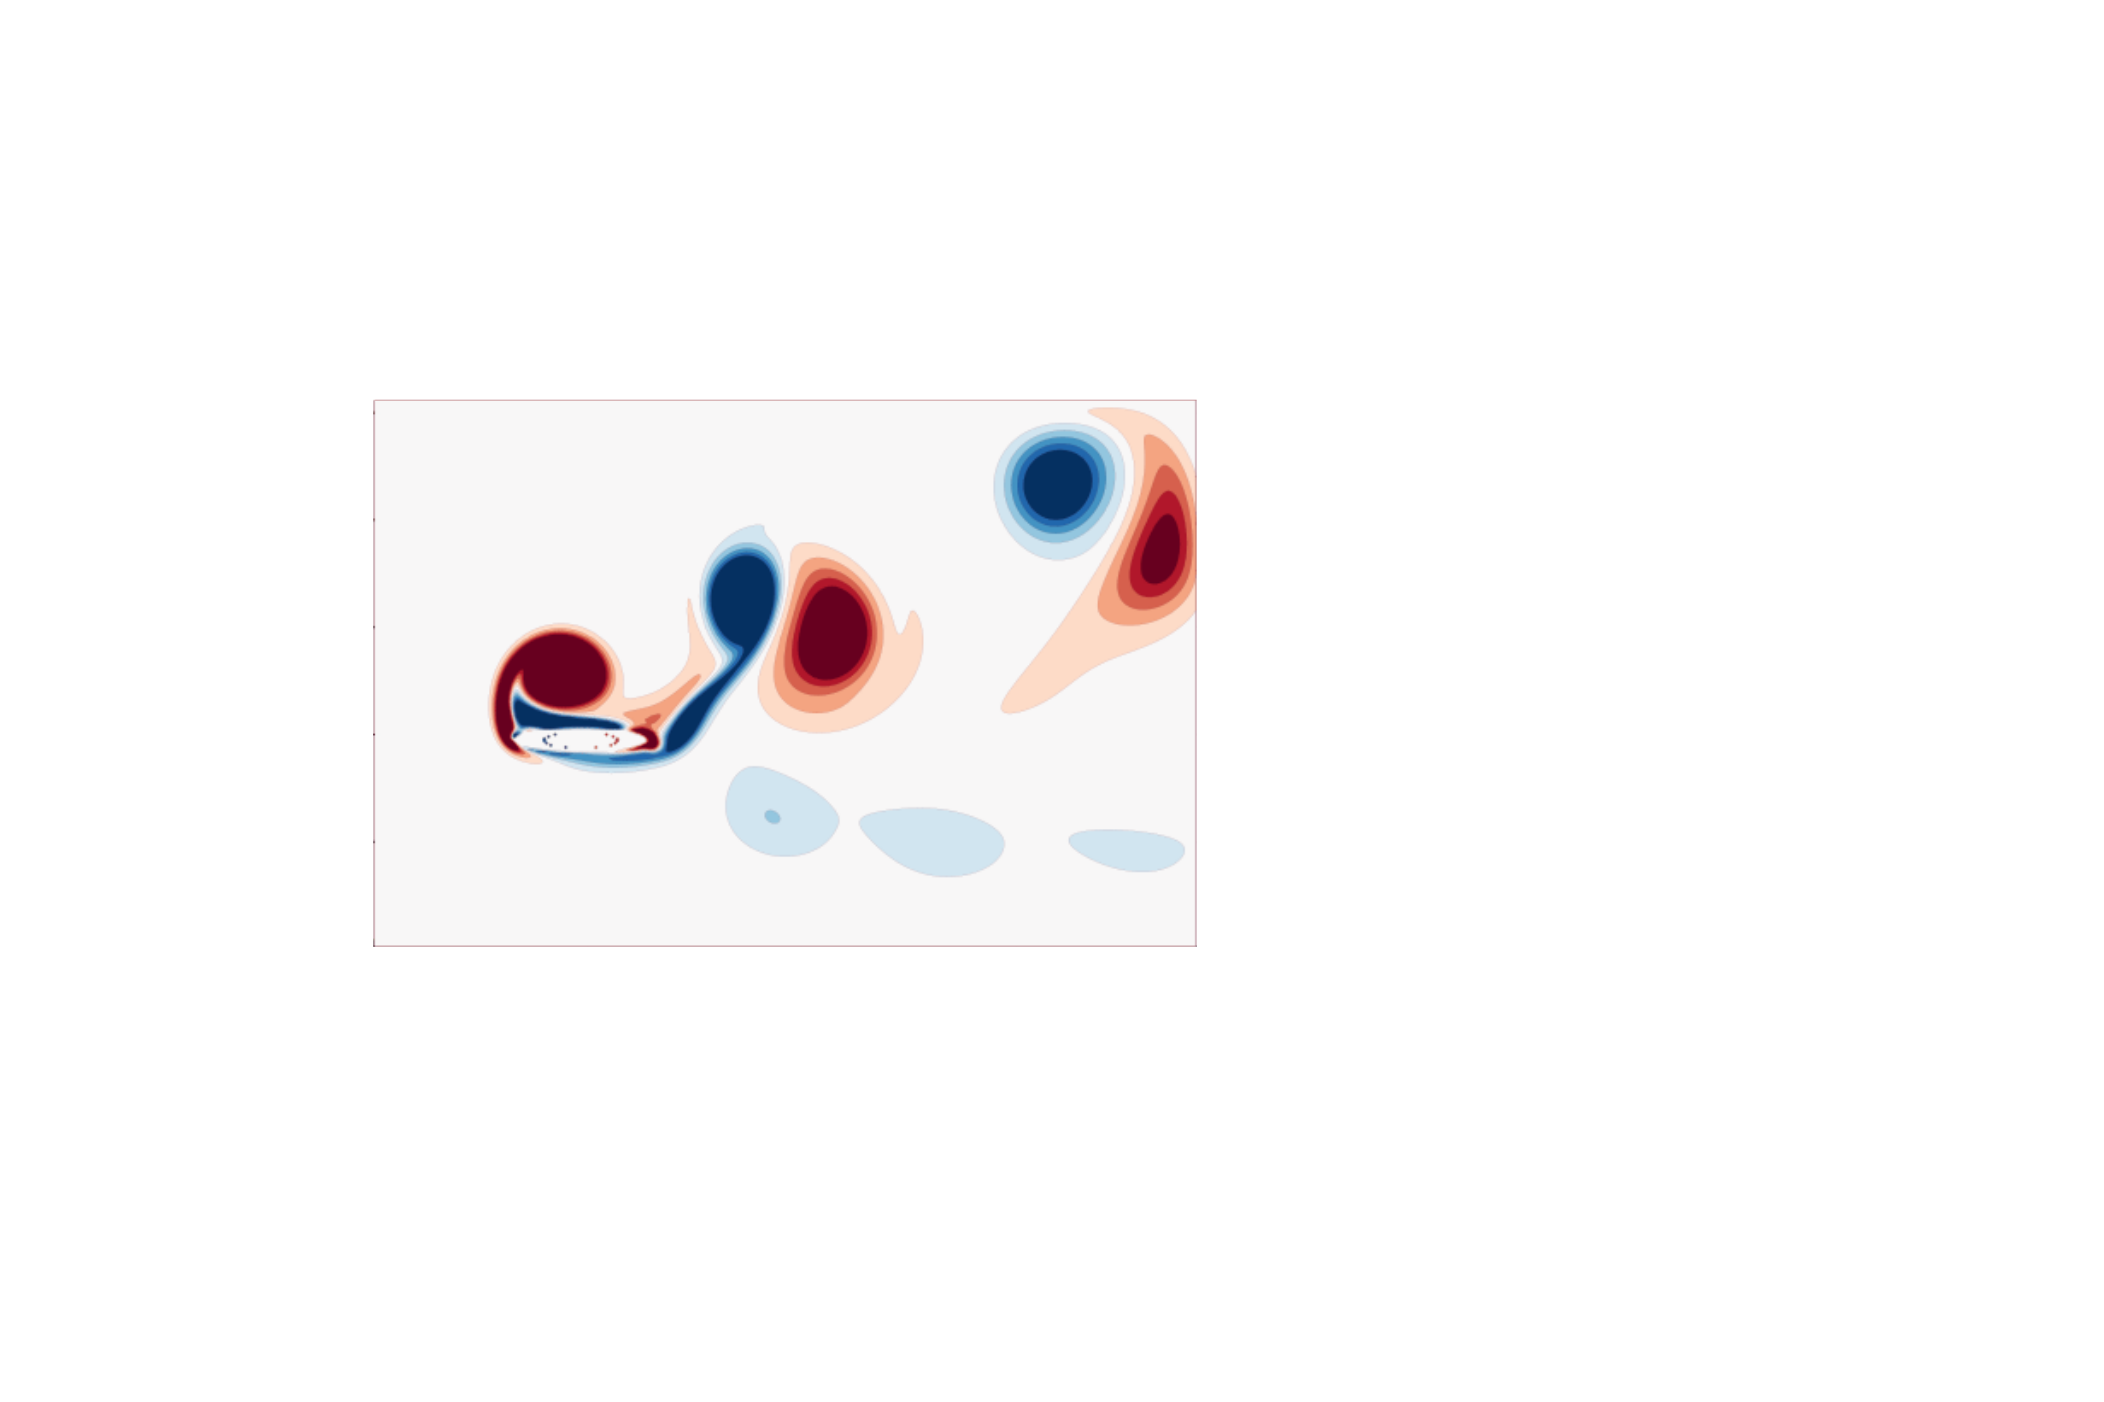
\includegraphics[trim={2.8cm 2cm 4cm 2cm},clip,width=\textwidth]{tex//fig/Deflected_wake_snap_BS.png}
        \caption{Biot-Savart ($6L\times4L$)}
    \end{subfigure}%
    \hspace{0.1cm}
    \begin{subfigure}{.48\textwidth}
        \centering
        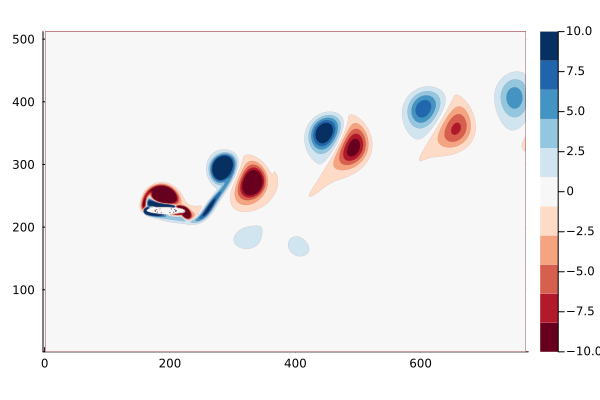
\includegraphics[trim={2.8cm 2cm 4cm 2cm},clip,width=\textwidth]{tex//fig/Deflected_wake_snap_BS_2x.png}
        \caption{\emph{Biot Savart} ($12L\times8L$)}
    \end{subfigure}
    \caption{Snapshot of the deflected wake behind an airfoil at $St=0.6$ and $Re=100$ for an amplitude to chord ratio $h_0/L=1.0$. The upper left panel $(a)$ shows the far wake obtained with the reflective boundary condition in a large domain, the upper right panel $(b)$ shows a zoom onto the airfoil and the near wake, the bottom left $(c)$ panel shows the entire (small) Biot-Savart domain used for the computation (the dashed line represents the domain boundaries) and the lower right panel $(d)$ shows the entire (larger) Biot-Savart domain. Vorticity is shown as 10 equally spaced isocontours in the interval $\omega L/U \pm 10$.}
    \label{fig:deflected_wake}
\end{figure}

Fig.~\ref{fig:deflected_wake} shows the vorticity field generated by the wing at $St=0.6$. The left panel shows the complete wake obtained with the large domain of size ($30L\times20L$). The left panel is a zoomed-in version of the same simulation, using a field of view with the size of the largest Biot-Savart domain. Finally, the bottom row shows two Biot-Savart simulations with two different domain sizes. The left panel shows the smallest domain of size ($6L\times4L$), represented by the gray dashed line, and the right panel shows a larger domain of size ($12L\times8L$) which extends to the whole panel.

Wake history strongly influences the near wake; the large domain correctly captures this, and a strong wake deflection is observed (the first vortex shed sets the direction; in this case, it is shed in the negative $y$ direction).

\begin{figure}
    \centering
    \begin{subfigure}{.5\textwidth}
        \centering
        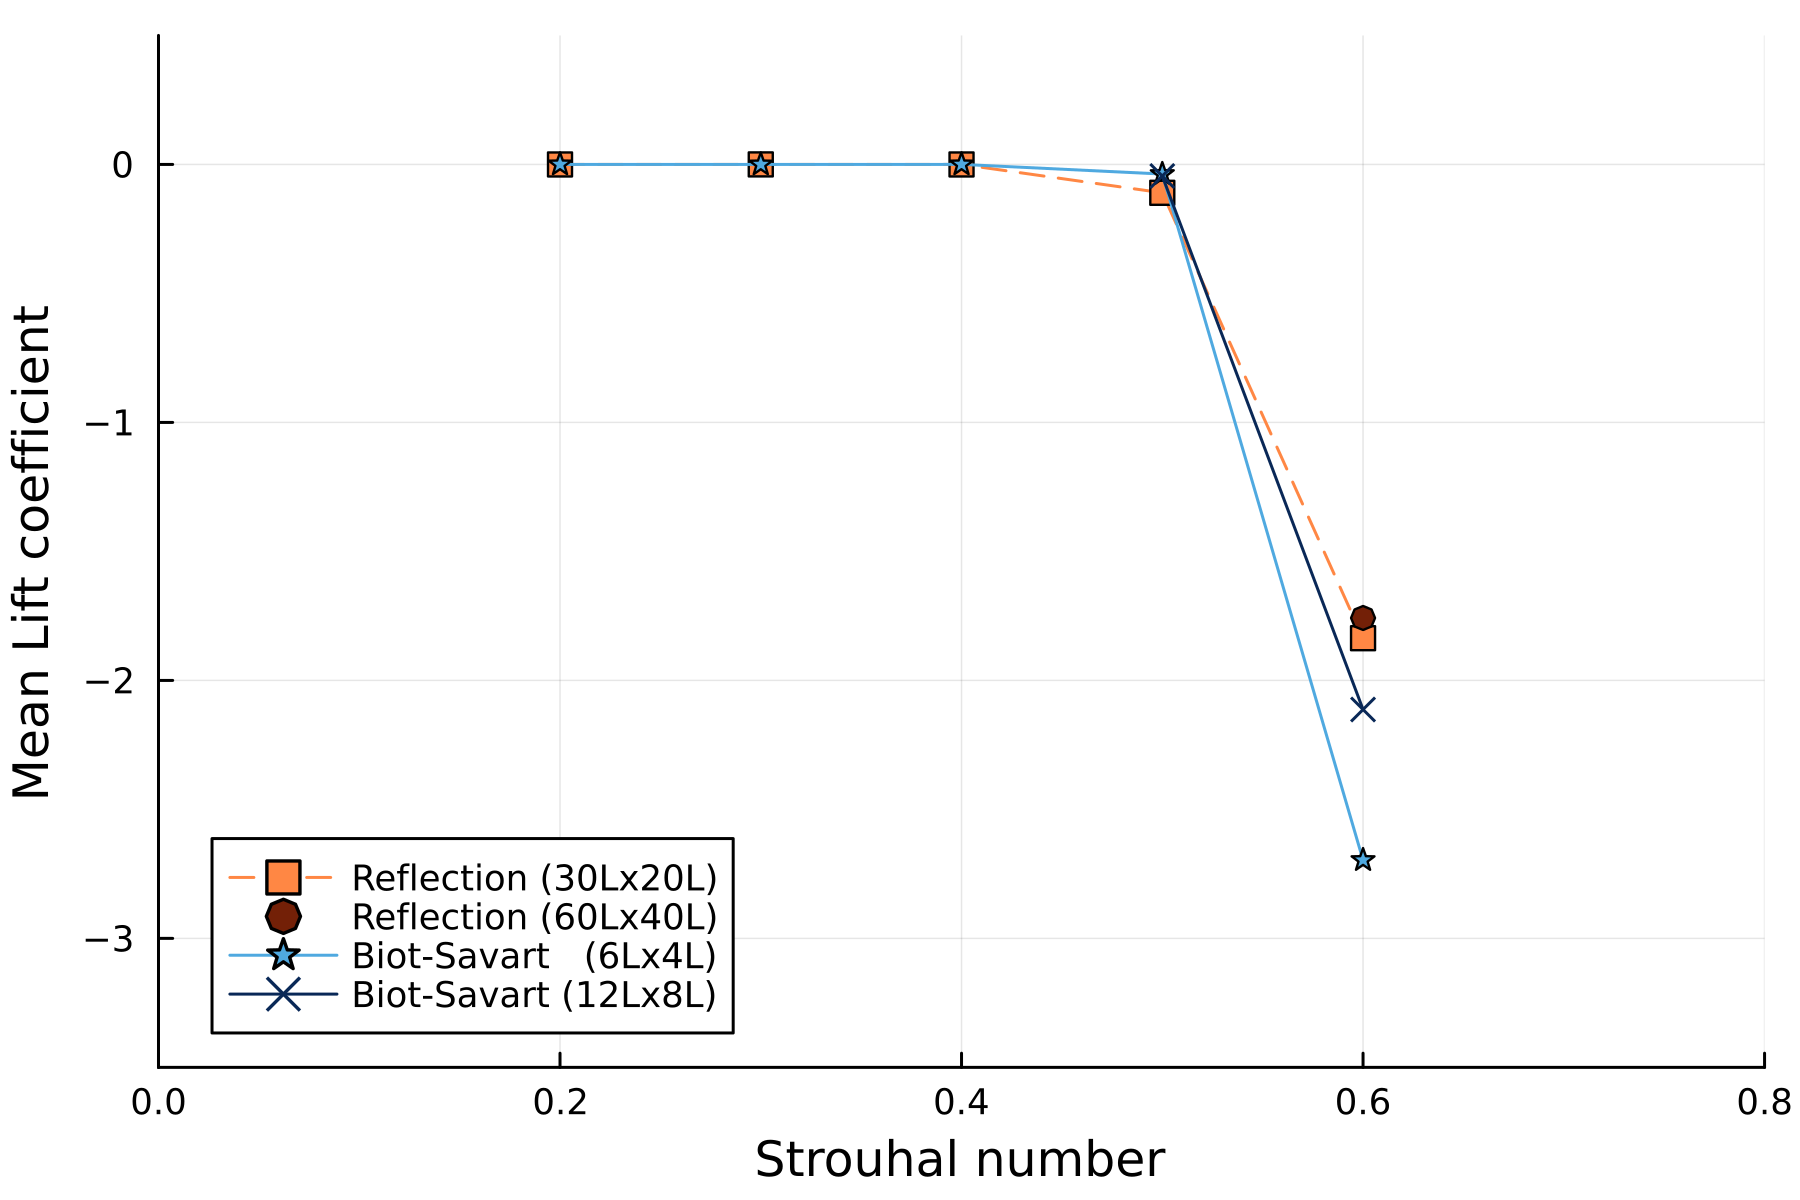
\includegraphics[trim={0 0 0 0},clip,width=\textwidth]{tex/fig/CL_mean_deflected_wake.png}
    \end{subfigure}%
    \begin{subfigure}{.5\textwidth}
        \centering
        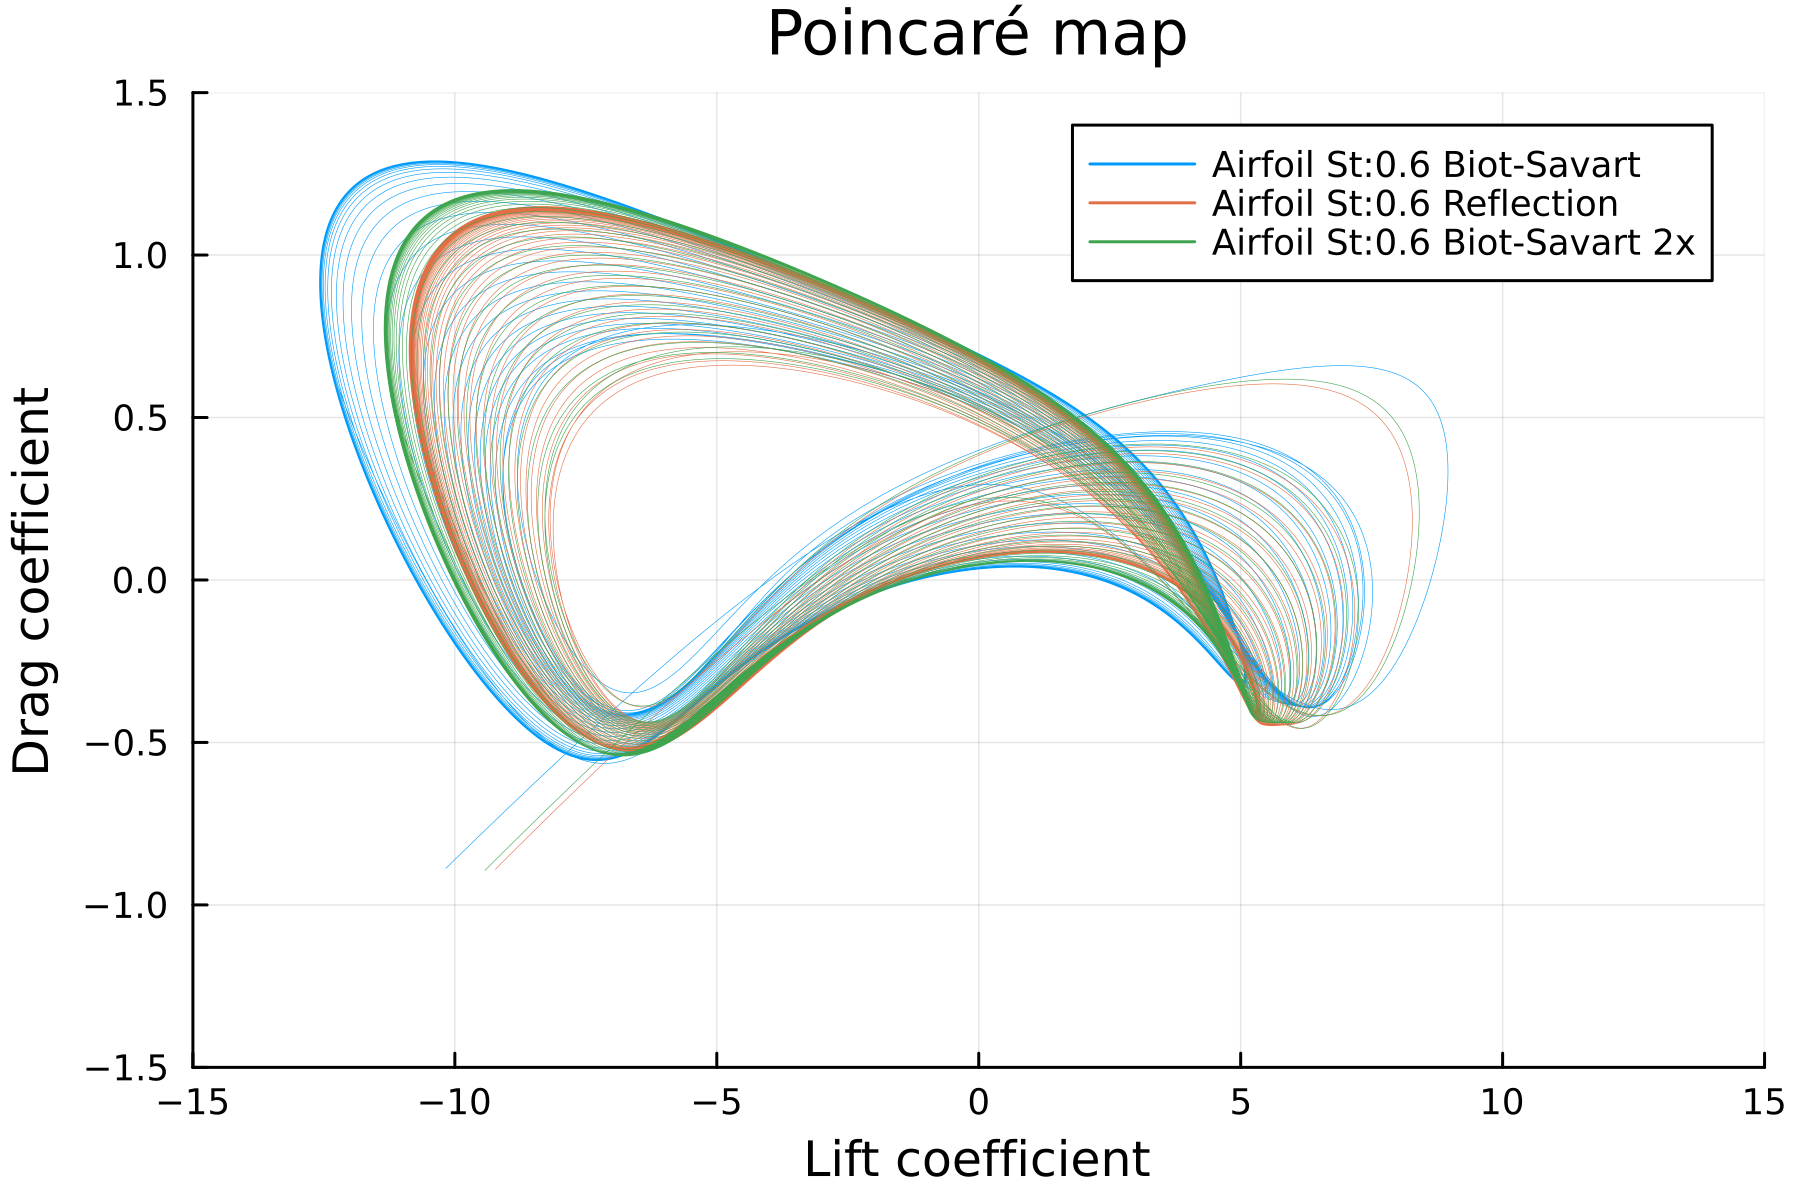
\includegraphics[trim={0 0 0 0},clip,width=\textwidth]{tex/fig/poincare_deflected_wake.png}
    \end{subfigure}
    \caption{(left) Mean lift force acting on the airfoil at $Re=100$, for a range of Strouhal numbers for the Biot-Savart and the reflective boundary condition  and (right) \emph{Poincar\'e} map of the lift and drag coefficients for $St=0.6$}
    \label{fig:deflected_wake_2}
\end{figure}

Without accurately accounting for this wake history by cutting the wake, this deflection is poorly captured, and the airfoil does not produce the typical large mean lift force associated with deflected wakes, see Fig.~\ref{fig:deflected_wake_2}. This high lift coefficient is generated from the high-velocity jets formed at the trailing edge of the airfoil (clearly observable on the right panels of Fig.\ref{fig:deflected_wake}), which are much weaker with our Biot-Savart boundary conditions on the small domain compared to classical reflective boundary conditions on the large domain or the larger Biot-Savart domain. While the small Biot-Savart domain fails to accurately capture the wake effects, doubling the domain size, while still using the Biot-Savart boundary conditions allows us to almost exactly recover the mean lift coefficient of the large domain and the reflective boundary conditions, see Fig~\ref{fig:deflected_wake_2}$b$. \emph{Poincar\'e maps} provide an excellent tool to examine the convergence of periodic orbits of dynamic systems. Fig.~\ref{fig:deflected_wake_2}$b$ shows such a map for the lift and drag coefficient of the heaving airfoil at $St=0.6$. The asymmetry in the lift, resulting in a net mean lift coefficient, is clearly observed for the larger domains (for both boundary conditions), while the small Biot-Savart domain shows almost perfectly symmetric orbits. For simulation where wake history effects are important, our Biot-Savart boundary condition required domains where this wake is allowed to be developed to accurately capture the resulting wake asymmetry and the large mean lift coefficients. 

While this is a limitation of our method, at least in terms of domain size, this flow is an artifact of 2D simulations and does not occur in actual flows. Indeed, experiments on finite foils have shown that these high-lift deflected jets cannot form for finite wings, see \cite{Calderon2014OnWings, Godoy-DianaTransitionFoil}.

 
\section{Conclusion}


In this manuscript, we presented a novel boundary condition formulation for the incompressible Navier-Stokes equations. The methods rely on a Biot-Savart integral of the vorticity inside the domain to set the velocity boundary conditions on the domain's boundaries. We couple these boundary conditions with an explicit projection scheme to solve the momentum and continuity equation in their primitive variables form. Leveraging the fast decaying properties of the Biot-Savart kernel, we use a multilevel algorithm to reduce the number of operations required to update the boundary nodes from $O(N)$ to $O(\log N)$ and show that the error introduced by this multilevel approach is bounded and can be estimated. We demonstrate that when a body is immersed in a domain using these boundary conditions, a coupling between the immersed body and the domain's boundary is introduced. This coupling only results in a weakly non-linear pressure Poisson equation and a simple differed correction approach can be used to solve the coupled projection/Biot-Savart step, allowing the use of standard Poisson solver.

With different examples of flow with confined vorticity, we show that the novel boundary conditions allow for a significant reduction in the size of the computational domain without any loss in accuracy. The method is able to exactly capture added-mass force on an accelerated disk with a computational domain only extending $1/2$ diameter away from the plate. 

Surprisingly, for vortex street applications, the method demonstrates its robustness and perfectly captures the drag forces and vortex shedding frequencies generated by a 2D circular cylinder at $Re=200$, even with minimal domain sizes ($5D\times3D$). Classical reflection boundary conditions requires a domain at least 10 times bigger to generate time-varying forces indistinguishable from that of the domain with our Biot-Savart boundary conditions. Lastly, we show that the method is limited when strong wake history influences the flow in the near wake. For a high-amplitude, high-Strouhal number heaving airfoil, we show that capturing the deflected wake of the flow requires significantly larger domain (with our Biot-Savart boundary conditions) and that the computational advantage is somewhat lost.

These results show that our novel boundary conditions are very effective for confined vorticity applications, such as accelerated bodies in the initial phase ($t^*<10$), when the vorticity is still confined to the body, or flow with very weak wake dependency.

% %% The Appendices part is started with the command \appendix;
% %% appendix sections are then done as normal sections
% \appendix

% \section{Sample Appendix Section}
% \label{sec:sample:appendix}

% Ultimately, we are interested in the magnitude of this error
% \begin{equation}
%     \varepsilon(\vec{x}) = \sum_{i=1}^{4}\vert\frac{\vec{\delta r}_i}{2\pi|\vec{r}|^2}\times\vec{e}_z\Gamma_i\vert = 
%     \sum_{i=1}^{4}\frac{\vert\vec{\delta r}_i\vert}{2\pi|\vec{r}|^2}\Gamma_i,
% \end{equation}
% as $\vec{e}_z$ does not contribute to the magnitude of the error. On uniform Cartesian meshes, we can relate the distance from the $i^{th}$ point-vortex to the cell center with the grid size on the $l$-level, $\vert\vec{\delta r}_i^{(l)}\vert=2^{l-3/2}$ (similarly in 3D we get $\vert\vec{\delta r}_i^{(l)}\vert=2^{l-3/2}\sqrt{3}$). The error introduced by the multilevel pooling of the vorticity field on the $l$-level is
% \begin{equation}
%     \varepsilon(\vec{x})^{(l)} = \sum_{i=1}^{4(l-1)}\frac{2^{l-3/2}}{2\pi|\vec{r}|^2}\Gamma_i.
% \end{equation}
% % \begin{equation}
% %     \varepsilon(\vec{x})^{(l)} = \sum_{i=1}^{4(l-1)}\frac{\sqrt{2}\Delta x}{4\pi|\vec{r}|^2}\Gamma_i=\frac{\sqrt{2}\Delta x}{4\pi|\vec{r}|^2}\sum_{i=1}^{4}\Gamma_i,
% % \end{equation}
% The level at which the vorticity is evaluated depends on the bounding box $\tilde{S}$ at each level. This criterion provides an upper bound for the error carried from level $l$ onto the induced velocity at $\vec x$ as $|\vec{r}|^2 \approx 2^{2l-2}\tilde{S}^2$ using Eq.~\eqref{eq:bbox}. The upper bound error is
% \begin{equation}
%     \varepsilon(\vec{x})^{(l)} = \frac{2^{l-3/2}}{2\pi\cdot2^{2l-2}\cdot\tilde{S}^2}\sum_{i=1}^{4(l-1)}\Gamma_i = \frac{2^{3/2}}{2^{l}\pi\tilde{S}^2}\sum_{i=1}^{4(l-1)}\Gamma_i.
% \end{equation}
% Finally, the upper bound for the total error in the induced velocity at a point $\vec x$ due to the $l$-level evaluation of the Biot-Savart integral is
% \begin{equation}
%     \varepsilon(\vec{x}) = \sum_{l=1}^{N_l}\frac{2^{3/2}}{2^{l}\pi\tilde{S}^2}\sum_{i=1}^{4(l-1)}\Gamma_i = \frac{2^{3/2}}{\pi\tilde{S}^2}\sum_{l=1}^{N_l}\frac{1}{2^l}\sum_{i=1}^{4(l-1)}\Gamma_i.
% \end{equation}
% which decays as $\tilde{S}^{-2}$. As expected, taking $\tilde{S}>\text{Domain}$ yields $\varepsilon(\vec{x}) = 0$, and as $\Gamma_i \to 0, \varepsilon(\vec{x})\to 0$, finally as $\tilde{S}\to0, \varepsilon(\vec{x}) \to \infty$. Similarly, in 3D the error is given by
% \begin{equation}
%     \varepsilon(\vec{x}) = \frac{2^{3/2}\sqrt{3}}{\pi\tilde{S}^3}\sum_{l=1}^{N_l}\frac{1}{2^{l}}\sum_{i=1}^{8(l-1)}\Gamma_i.
% \end{equation}
% which decays as $\tilde{S}^{-3}$. 

%% If you have bibdatabase file and want bibtex to generate the
%% bibitems, please use
%%
 \bibliographystyle{elsarticle-num} 
 \bibliography{references}

%% else use the following coding to input the bibitems directly in the
%% TeX file.

% \begin{thebibliography}{00}

% %% \bibitem{label}
% %% Text of bibliographic item

% \bibitem{}

% \end{thebibliography}
\end{document}
\endinput
%%
%% End of file `elsarticle-template-num.tex'.
